% !TeX encoding = UTF-8
\documentclass[red, % Color red
tikz, 
%aspectratio=169, % wide slide
xcolor=table]{beamer}

% ATENÇÃO, READ-ME, LEIA AQUI
% O PACOTE tikzpicture NÃO ESTÁ COMPILANDO NO OVERLEAF E POR ISSO
% DEVE SER COMPILADO LOCALMENTE POIS É SUCESSO
% DEIXAR A CÓPIA NO GIT MESMO ASSIM POR BACKUP

%%%%%%%%%%%%%%%% Theme
\setbeamertemplate{blocks}[rounded][shadow=false] %blocks rounded
\usetheme{Madrid} % theame name
\setbeamertemplate{items}[square] % items squared
\setbeamertemplate{itemize item}{\color[rgb]{0.8,0,0}$\blacksquare$}
\setbeamertemplate{itemize subitem}{\color[rgb]{0.8,0,0}$\blacksquare$}
\setbeamertemplate{itemize subsubitem}{\color[rgb]{0.8,0,0}$\blacksquare$}
\setbeamertemplate{caption}[numbered] 
\usecolortheme{beaver}
\setbeamercolor{frametitle}{bg=white!10!white}

%%%%%%%%%%%%%%%% For notations in speaker time
% Para comentários no presentation.app
\usepackage{pdfcomment}
\newcommand{\pdfnote}[1]{\marginnote{\pdfcomment[icon=note]{#1}}}

%%%%%%%%%%%%%%%% Fonts
\usefonttheme{professionalfonts}

%%%%%%%%%%%%%%%% Definições de seção
\setcounter{secnumdepth}{3}
\setcounter{tocdepth}{2}

\mode<presentation>{} % https://tex.stackexchange.com/questions/116913/display-the-definition-of-each-items-in-beamer-one-by-one-using-onslide-or-any-m
\usepackage{textcomp}
\usepackage{xkeyval}
\usepackage{todonotes}
\presetkeys{todonotes}{inline}{}

\usepackage{tikzsymbols}
\usepackage{tikz}
\tikzset{
   invisible/.style={opacity=0},
   visible on/.style={alt={#1{}{invisible}}},
   alt/.code args={<#1>#2#3}{%
      \alt<#1>{\pgfkeysalso{#2}}{\pgfkeysalso{#3}} % \pgfkeysalso doesn't change the path
   },
}

\usepackage{pgfplots}
\usepackage{helvet}
\renewcommand{\familydefault}{\sfdefault}
\usepackage{float}
\usepackage[brazil]{babel}
\usepackage[utf8]{inputenc}
\usepackage{graphicx}
\usepackage{url}
\usepackage{subfigure}
\usepackage{mathtools} % setas com texto
\usepackage{multicol}
\usepackage{listings}
\usepackage{scalefnt}
\usepackage{ragged2e}
\usepackage{etoolbox, verbatim}
\usepackage{soul}

\usepackage{tabularx,booktabs,dcolumn} %tabela
\usepackage{ltablex}
\newcommand{\specialcell}[2][c]{\begin{tabular}[#1]{@{}c@{}}#2\end{tabular}}

\usepackage{pifont}% http://ctan.org/pkg/pifont
\newcommand{\cmark}{\ding{51}}%
\newcommand{\xmark}{\ding{55}}%

\usepackage[linguistics]{forest}
\usepackage[cache=false]{minted}

\usepackage{amsmath}
\usepackage[algoruled,linesnumbered,lined,portuguese]{algorithm2e}

\newcommand{\hardware }{\textit{hardware}}
\newcommand{\Hardware }{\textit{Hardware}}
\newcommand{\software }{\textit{software}}
\newcommand{\Software }{\textit{Software}}
\newcommand{\hardwares}{\textit{hardwares}}
\newcommand{\Hardwares}{\textit{Hardwares}}
\newcommand{\softwares}{\textit{softwares}}
\newcommand{\Softwares}{\textit{Softwares}}

\newcommand{\hs}{\textit{hardware}\ e\ \textit{software}}
\newcommand{\HS}{\textit{Hardware}\ e\ \textit{Software}}

\newcommand{\wearable} {\textit{wearable}}
\newcommand{\Wearable} {\textit{Wearable}}
\newcommand{\wearables}{\textit{wearables}}
\newcommand{\Wearables}{\textit{Wearables}}


\newcommand{\design}   {\textit{design}}
\newcommand{\designer} {\textit{designer}}
\newcommand{\Design}   {\textit{Design}}
\newcommand{\Designer} {\textit{Designer}}
\newcommand{\designs}  {\textit{designs}}
\newcommand{\designers}{\textit{designsers}}
\newcommand{\Designs}  {\textit{Designs}}
\newcommand{\Designers}{\textit{Designers}}
\newcommand{\assembly} {\textit{assembly}}
\newcommand{\profile}  {\textit{profile}}
\newcommand{\Profile}  {\textit{Profile}}
\newcommand{\speedup}  {\textit{speedup}}
\newcommand{\Speedup}  {\textit{Speedup}}
\newcommand{\core}     {\textit{core}}
\newcommand{\cores}    {\textit{cores}}
\newcommand{\codesign} {\textit{codesign}}
\newcommand{\mobile}   {\textit{mobile}}
\newcommand{\benchmark}   {\textit{benchmark}}
\newcommand{\benchmarks}   {\textit{benchmarks}}
\newcommand{\Benchmark}   {\textit{Benchmark}}
\newcommand{\Benchmarks}   {\textit{Benchmarks}}
\newcommand{\titulo}{Uma Abordagem do Problema de Particionamento \textit{Hardware} e \textit{Software} para \textit{Design} de Sistemas Computacionais \textit{Wearables}}

\newcommand{\bx}[1]{\colorbox{yellow}{\fbox{#1}}}

\newcommand{\Abs}[1]{\left\lvert#1\right\rvert}

\newcommand{\A}{$\mathcal{A}$}
\newcommand{\B}{$\mathcal{B}$}
\newcommand{\C}{$\mathcal{C}$}

\definecolor{beamerVermelho}{RGB}{162, 0, 0}
\definecolor{beamerCinza}{RGB}{101, 101, 101}

%\usepackage[natbib=true, bibstyle=authoryear, citestyle=authoryear-comp]{biblatex}
%\usepackage{natbib}%\bibpunct{(}{)}{;}{a}{,}{,}

% Listing
\lstset{
	numbers=left,
	stepnumber=1,
	numbersep=5pt,
	numberstyle=\small\color{black},
	basicstyle= \scriptsize,
%	keywordstyle=\color{black},
%	commentstyle=\color{black},
%	stringstyle=\color{black},
	tabsize=2
}

\let\olditem=\item%
%\renewcommand{\item}{\olditem \justifying} % texto justificado

\title[Universidade Federal de Ouro Preto (UFOP)]{\textbf{\titulo}\\}

\author[\textit{rodolfolabiapari@decom.ufop.br}]{
   Discente: Rodolfo Labiapari Mansur Guimarães \\ Orientador: Dr. Ricardo Augusto Rabelo Oliveira}

\institute[UFOP]{\begin{figure}
			\centering
			
\includegraphics[width=0.1\textwidth]{img/ufop.jpg}
		\end{figure}}
   
\institute[]{
	\textit{rodolfolabiapari@decom.ufop.br} -- Lattes: \url{http://goo.gl/MZv4Dc} \\
	Departamento de Computação -- Instituto de Ciências Exatas e Biológicas (DECOM-ICEB)\\
	Universidade Federal de Ouro Preto (UFOP) \\
	Ouro Preto - MG -- Brasil }

\date[\today]{Última Atualização: \today}

%\usepackage{bibentry}

\usepackage[backend=bibtex, firstinits=true, style=alphabetic,maxalphanames=1]{biblatex}
\addbibresource{bibliography.bib}
% Removes icon in bibliography
%\setbeamertemplate{bibliography item}{}


\usepackage{appendixnumberbeamer} % appendix stop count

\begin{document}

\frame{\titlepage}

%\AtBeginSection[]
%{
\begin{frame}
	\frametitle{Sumário}
	\tableofcontents[hideallsubsections]
\end{frame}
%}


\usebackgroundtemplate{
\includegraphics[trim=0cm 0cm 2cm -393cm, width=0.03\textwidth]{img/ufop.jpg}}

% !TeX encoding = UTF-8
% !TEX root = ./presentation.tex
\section{Apresentação}

   \subsection{Introdução ao Problema}
      \begin{frame}
         \frametitle{Introdução}
         \begin{itemize}
            \setlength{\itemsep}{1.3em}
            \item Sistemas embarcados (SE) e \wearables\ estão cada vez mais presentes, devido
            \begin{itemize} \setlength{\itemsep}{0.3em}
               \item Progresso na \textbf{obtenção} e \textbf{manipulação de informações};
               \item \textbf{Ascensão da tecnologia} da microeletrônica, comunicação e sensores \cite{Jozwiak2017}.
            \end{itemize}
            
            \item Demanda por \textbf{curto tempo para disponibilidade} ao mercado;
            \item Propriedades de \textbf{corretude}, \textbf{rapidez}, \textbf{confiabilidade} e \textbf{preço acessível}.
            
            
            \item SE gerais são considerados únicos pela necessidade de um \codesign\ \cite{Wolf1994}
            \begin{itemize}
               
               \item Possuem componentes \textbf{implementados tanto em \hs}.
            \end{itemize}
            
         \end{itemize}
         \pdfnote{As pesquisas em \codesign\ têm como objetivo o \design\ de sistemas heterogêneos, visando performance, custo e metas de confiabilidade \cite{Edwards1994}}
      \end{frame}
      

      \begin{frame} \vspace{-1em}
         \frametitle{Problema de Particionamento}
         \begin{itemize} \setlength{\itemsep}{1.6em}
            \item Preocupação atual no desenvolvimentos de projetos SE
            \begin{itemize} \setlength{\itemsep}{1.2em}
               \item A \textbf{redução do ciclo de comercialização} de um produto;
               \item Aumento de sua \textbf{eficiência}.
            \end{itemize}
            
            
            \item Sobre isso, o particionamento \hs
            \begin{itemize} \setlength{\itemsep}{1.2em}
               \item \cite{Hassine2017}: ``uma das \textbf{soluções mais elegantes} na computação que provê \textbf{otimizações sistêmicas} sobre essas circunstâncias'';
               \item Ou seja, uma das \textbf{principais tecnologias para o desenvolvimento de sistemas embarcados em geral}.
            \end{itemize}
            
         \end{itemize}
      \end{frame}
      
      
      
   \subsection{Motivação}
      \begin{frame} \vspace{-1em}
         \frametitle{Motivação}
         \begin{itemize} \setlength{\itemsep}{1.2em}
            \item Produtos modernos \textbf{necessitam} de um bom \codesign\ \cite{Trappey2016}. 
            
            \item Implementações somente em módulos de \software
            \begin{itemize}
               \item Possuem \textbf{mais flexibilidade} e são \textbf{menos custosos};
               \item Entretanto, seu custo \textbf{eleva-se} em termos de \textbf{tempo de execução};
            \end{itemize}
           
            \item Ao utilizar recursos em \hardware\ \cite{Zhang2008, Hassine2017, Wolf1994, Canis2011, Stone2010}
            \begin{itemize}
               \item Proverá maior \textbf{eficiência energética}; e 
               \item \textbf{\Speedup}\ maior às implementações.
            \end{itemize}
            
                  
            % combinação de fpga com cpu
            \item Processador + \hardware\ reconfigurável\footnote{FPGAs, do inglês \textit{Field-Programmable Gates Array}.} forma um sistema computacional híbrido
            
            \begin{itemize}
               \item Utilizado como meio para melhoria de desempenho e eficiência energética \cite{Cong2009, Lo2009, Zhang2008a}. 
            \end{itemize}
            
         \end{itemize}
         
      \end{frame}
   
   
   \subsection{Objetivos}
      \begin{frame}{Objetivos}
      
         \begin{itemize} \setlength{\itemsep}{1.2em}
            \item \textbf{Gerais}
            \begin{itemize} \setlength{\itemsep}{0.6em}
               \item Abordagem do particionamento \hs;
               \item Sua importância no mundo de sistemas computacionais embutidos, foco em sistemas \wearables.
            \end{itemize}
            
            \item \textbf{Específicos}
            
            \begin{itemize} \setlength{\itemsep}{0.6em}
               \item Apresentação do problema de particionamento \hs\ com foco em sistemas \wearables;
               
               \item Principais soluções apresentadas ao logo dos anos e as utilizadas atualmente;
               
               \item  Ferramentas \textit{high-level syntesis} (HLS) como LegUp e OpenCL para a geração de sistemas computacionais que usufruem de aceleradores em \hardware.
               
               \item Abordagem metodológica para a procura da solução do problema de particionamento \hs\ apresentado.
            \end{itemize}
         \end{itemize}
         
      \end{frame}
      
      \begin{frame}{Processos} \vspace{-1em}
         \begin{itemize} \setlength{\itemsep}{1.2em}
            \item \textbf{Justificativa:}
            \begin{itemize} \setlength{\itemsep}{0.3em}
               \item \Designs\ mais complexos.
               
               \item Necessidade de eficiência energética segue junto com \speedup\ \cite{Trindade2016, Arato2005, Yan2017}.
               
               \item Defasagem em pesquisa científica para \wearables.
               
            \end{itemize}
         
            \item \textbf{Objetivo:} 
            \begin{itemize} \setlength{\itemsep}{0.3em}
               \item \textbf{Balanceamento de todas as tarefas} otimizando alguns objetivos de sistema sobre determinadas restrições.
               
               \item \textbf{Alta performance} com o \textbf{baixo consumo de energia} para maximizar o tempo de uso da bateria.
            \end{itemize}
            \item \textbf{Metodologia:} 
            \begin{enumerate} \setlength{\itemsep}{0.3em}
               \item Agrupar específicos conjuntos de instruções de uma aplicação; e
               \item Mapear esses grupos tanto em \hs.
            \end{enumerate}
         
            \item \textbf{Contribuição Esperada:} 
            \begin{itemize} \setlength{\itemsep}{0.3em}
               \item Pesquisa sobre \wearables.
            \end{itemize}
         \end{itemize}
      \end{frame}
 


\AtBeginSubsection[]
{
   \begin{frame}
      \frametitle{Sumário}
      \tableofcontents[
      currentsection,
      %sectionstyle=show/hiden,
      %currentsubsection,
      hideothersubsections,
      %subsectionstyle=show/shaded, 
      ]
   \end{frame}
}

%% !TeX encoding = UTF-8
% !TEX root = ./presentation.tex
\section{Referencial Teórico}
   \subsection{{\it Field-Programmable Logic Device} (FPGA) e Recursos}
      %\frame{\centering \bf \Huge \color{beamerCinza} \textit{Field-Programmable Logic Device}}
      % uso de fpga no mundo
      
      \begin{frame}{\textit{Field-Programmable Logic Device} (FPGA)}
         \begin{figure}[h] \centering
            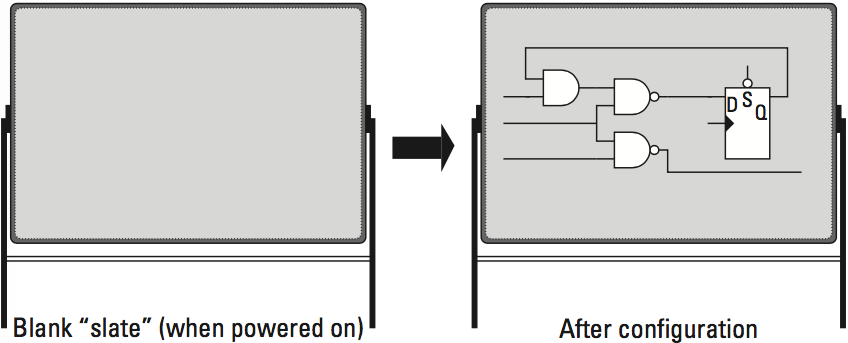
\includegraphics[width=1\textwidth]{img/rt-board.png}
            \caption{Ilustração em alto nível do funcionamento interno do FPGA. Fonte: \cite{Sass2010}.}
         \end{figure}
         \pdfnote{explicar titulo}
         \pdfnote{pode ser configurados facilmente}
         \pdfnote{linguagem ainda complexa}
      \end{frame}
   
      \begin{frame}{\textit{Field-Programmable Logic Device} (FPGA)} \vspace{-1.3em}
         \begin{figure}[h] \centering
            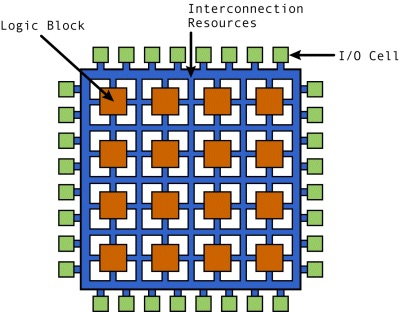
\includegraphics[width=0.75\textwidth]{img/rt-arch_fpga.jpg}
            \caption{Exemplo da arquitetura internas de um FPGA. Fonte: \url{http://www.eetimes.com/document.asp?doc_id=1274496}. Acesso: 30/05/2017.}
         \end{figure}
         \pdfnote{Tornando-o um dos (CI) MAIS densos existente.}
      \end{frame}
      
      \begin{frame}{\textit{Field-Programmable Logic Device} (FPGA)}{Introdução} \vspace{-1em}
         \begin{itemize}
            \setlength{\itemsep}{1.5em}
            \item FPGAs eram utilizados unicamente na protitipação ASIC.
            
            \item Mas com a \textbf{elevação do custo} de pesquisa, \design, desenvolvimento e teste de um novo produto
            \begin{itemize}\setlength{\itemsep}{0.5em}
               \item Interessou-se na utilização de FPGAs \cite{Mei2000};
               \item Vantagens em termos de flexibilidade de projeto.
            \end{itemize}
            
            \item Entretanto \cite{Sass2010}
            \begin{itemize}\setlength{\itemsep}{0.5em}
               \item + Configurar um \hardware\ reconfigurável é uma tarefa fácil graças às ferramentas disponíveis hoje;
               
               \item - \textbf{criar um \design\ de \hardware\ inicial não é}.
            \end{itemize}
            
         \end{itemize}
      \end{frame}
   
   
      \begin{frame}{FPGA + Processadores}{\textit{Hard} e \textit{Software Cores} \cite{Plessl2003}} \vspace{-1em} 
         \begin{itemize}
            \setlength{\itemsep}{0.5em}
            \item \textbf{\textit{Hard Core}:} \core\ dedicado;
            \item \textbf{\textit{Soft Core}:} sintetizado e mapeado no FPGA com seus recursos lógicos. 
         \end{itemize}
      
         \begin{figure}[h] \centering
            \vspace{-8pt}
            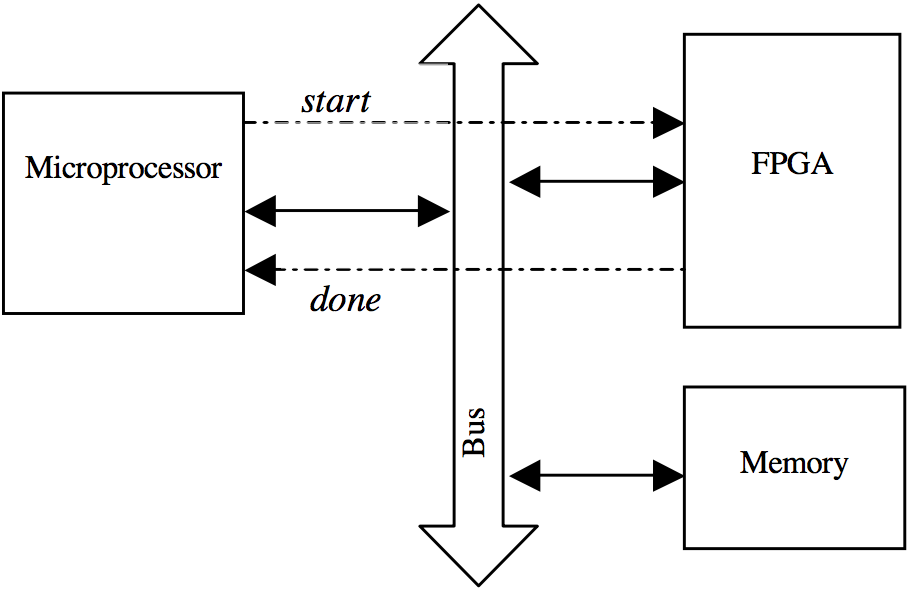
\includegraphics[width=0.7\textwidth]{img/into-soc.png}
            \caption{Visão geral de um SoC FPGA.}
            \label{fig:rb-soc}
         \end{figure}
      
         \pdfnote{HC: um pedaço de CI dentro (ou não) de um FPGA}
         \pdfnote{SC: é obtido por meio de \design\ e sintetização na placa }
         \pdfnote{vantags:}
         \pdfnote{usar todos recursos, máxima performance}
         \pdfnote{permite a extensão da arquitetura}
         \pdfnote{-> HDL}
      \end{frame}
   
      \begin{frame}{\textit{Hardware Description Language} (HDL)} \vspace{-1em}
         \begin{itemize}
            \setlength{\itemsep}{1.0em}
            \item \textbf{Classes de linguagens} de computação usados para \textbf{descrever formalmente um circuito eletrônico}.
            \begin{itemize}
               \item Pois possui detalhação altíssima do \hardware.
            \end{itemize} 
            
            \item Descreve o \cite{Sass2010}
            
            \begin{itemize}
               \item \textbf{Comportamento temporal}; ou a 
               \item \textbf{Estrutura de circuito espacial} de um sistema eletrônico.
            \end{itemize}
         
            \item Vantagens \cite{Smith1998}. 
            \begin{itemize}
               \item Pode-se \textbf{alterar} o código HDL, \textbf{e sintetizar no mesmo dispositivo} para testar;
               \item \textbf{Quantas vezes forem necessárias}, \textbf{sem custo adicional}.
            \end{itemize}
            
            \item Desvantagem
            \begin{itemize}
               \item - \textbf{Nível elevado de complexidade} de programação  \cite{Choi2016};
               \item + Existe outras linguagens disponíveis para uso \cite{Sass2010}. 
            \end{itemize}
         \end{itemize}
      \end{frame}
   
   
      \begin{frame}{\textit{High-Level Synthesis} (HLS)} \vspace{-1em}
         \begin{itemize}
            \setlength{\itemsep}{0.9em}
            \item Sintetizam códigos de alto nível para HDLs \cite{Choi2016} \cite{Trevett2008}
            \begin{itemize}
               \setlength{\itemsep}{0.2em}
               \item \textbf{Reduzir} os longos ciclos do \textbf{processo de \design}\ de \hardware; e ainda
               \item Traz \textbf{melhoria em performance e eficiência energética};
               \item Entrega um bom HDL.
            \end{itemize}
            
               \bigskip
            
            \item LegUp High-Level Synthesis
            \begin{itemize}
               \setlength{\itemsep}{0.2em}
               \item \textbf{Entrada:} código padrão \textit{C};
               \item \textbf{Saída:} compilação para dispositivos FPGA \cite{Canis2011};
               \item \textbf{Pode gerar:} \textit{hard} e \textit{soft cores};
            \end{itemize}
           
            \item OpenCL
            \begin{itemize}
               \setlength{\itemsep}{0.2em}
               \item API para \textbf{execução de programas em sistemas heterogêneos}
               \begin{itemize}
                  \item Processadores \textit{multicores}, GPUs ou outros aceleradores \cite{Shagrithaya2013, Czajkowski2012}. 
               \end{itemize}
               
               \item Nível de \textbf{paralelismo em tarefas e dados}.
               
            \end{itemize}
            \pdfnote{bib \textit{multi-threads} \textit{Pthread}, \textit{OpenMP} aceler. }
            
         \end{itemize}
      \end{frame}
   
      \begin{frame}[fragile]{}
         \begin{minted}[mathescape,
         linenos,
         fontsize=\tiny,
         framesep=2mm]{c}
void fourn(float data[], unsigned long nn[], int ndim, int isign) {
   for (ntot = 1, idim = 1; idim <= ndim; idim++) ntot *= nn[idim]; nprev = 1;
   for (idim = ndim; idim >= 1; idim--) {
      n = nn[idim]; nrem = ntot / (n * nprev);
      ip1 = nprev << 1; ip2 = ip1 * n; ip3 = ip2 * nrem; i2rev = 1;
      for (i2 = 1; i2 <= ip2; i2 += ip1) {
         if (i2 < i2rev) {
            for (i1 = i2; i1 <= i2+ip1-2; i1 += 2) {
               for (i3 = i1; i3 <= ip3; i3 += ip2) {
                  i3rev = i2rev + i3 - i2;
                  SWAP(data[i3], data[i3rev]); SWAP(data[i3+1], data[i3rev + 1]);
               }
            }
         }  ibit = ip2 >> 1;
         while (ibit >= ip1 && i2rev > ibit) { i2rev -=  ibit; ibit >>=  1; }
         i2rev += ibit;
      } ifp1 = ip1;
      while (ifp1 < ip2) {
         ifp2 = ifp1 << 1; theta = isign * 6.28318530717959 / (ifp2 / ip1);
         wtemp = sin(0.5 * theta);  wpr = -2.0 * wtemp * wtemp;
         wpi = sin(theta); wr = 1.0; wi = 0.0;
         for (i3 = 1; i3 <= ifp1; i3 += ip1) {
            for (i1 = i3; i1 <= i3 + ip1 - 2; i1 +=  2) {
               for (i2 = i1; i2 <= ip3; i2 +=  ifp2) {
                  k1 = i2; k2 = k1 + ifp1;
                  tempr = (float) wr * data[k2] - (float) wi * data[k2 + 1];
                  tempi = (float) wr * data[k2 + 1] + (float) wi * data[k2];
                  data[k2] = data[k1] - tempr;
                  data[k2 + 1] = data[k1 + 1] - tempi;
                  data[k1] += tempr; data[k1+1] += tempi;
               }
            } wr = (wtemp = wr) * wpr - wi * wpi + wr;
            wi = wi * wpr + wtemp * wpi + wi;
         } ifp1 = ifp2;
      } nprev *= n; 
   } }
         \end{minted}
\end{frame}

      \begin{frame}[fragile]{LegUp Processos}
         \begin{minted}{shell}
source ../legup.tcl
set_project CycloneV SoCKit ARM_Simple_Hybrid_System

set_accelerator_function "fourn"
\end{minted}
         \pause
         \vspace{2em}
         
         \begin{figure}
            \begin{tikzpicture}[auto, node distance=3.5 cm, >=latex']
            %\tikzstyle{block}    = [draw, rectangle, minimum height=2em, minimum width=4em, fill=red!20]
            %\tikzstyle{input}    = [coordenate]
            %\tikzstyle{output}   = [coordenate]
            %\tikzstyle{pinstyle} = [pin edge={to-,thin,black}]
            \matrix[column sep = .75cm, row sep = .375cm]{
               \node[draw, shape=rectangle, fill=red!20, visible on=<1->] (c)      {C Code}; & & \\
               &
               \node[draw, shape=rectangle, fill=red!20, visible on=<2->] (hdl)    {Generates HDL Code};&
               \node[draw, shape=rectangle, fill=red!20, visible on=<3->] (synth)  {Synthesizes it}; \\
               \node[draw, shape=rectangle, fill=red!20, visible on=<1->] (config) {Config File};& & \\
            }; 
            \draw [->, thick, visible on=<1->] (c) -- (hdl);
            \draw [->, thick, visible on=<1->] (config) -- (hdl);
            \draw [->, thick, visible on=<2->] (hdl) -- (synth);
            \end{tikzpicture}
            \caption{Processo de geração de código por meio do LegUp HLS.}
         \end{figure}
         
\end{frame}
   
      \begin{frame}[fragile]{OpenCL}
         \begin{minted}{c}
__kernel void
vectorAdd(__global const float * a,
          __global const float * b,
          __global       float * c) {
   // Indice do vetor
   int nIndex = get_global_id(0);
   
   c[nIndex] = a[nIndex] + b[nIndex];
}
         \end{minted}
\end{frame}
      
      \begin{frame}{OpenCL} \vspace{-1em}
         \begin{figure}[h] \centering
         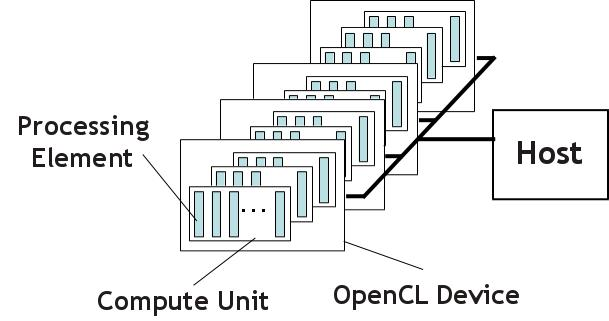
\includegraphics[width=1\textwidth]{img/opencl.jpg}
         \caption{Sistema hierárquico de um projeto em OpenCL. Fonte: \url{https://handsonopencl.github.io/} Acessado em: 07/08/2017.}
         \label{fig:opencl}
         \end{figure}
      \end{frame}


   
   \subsection{Ferramenta {\it Profile}}
   %\frame{\centering \bf \Huge \color{beamerCinza} \textit{Profile}}

      \begin{frame}{\textit{Profile}} \vspace{-1em}
         
         \begin{columns}
            \begin{column}{0.5\textwidth}
               
               \begin{figure}[h] \centering
                  \vspace{-24pt}
                  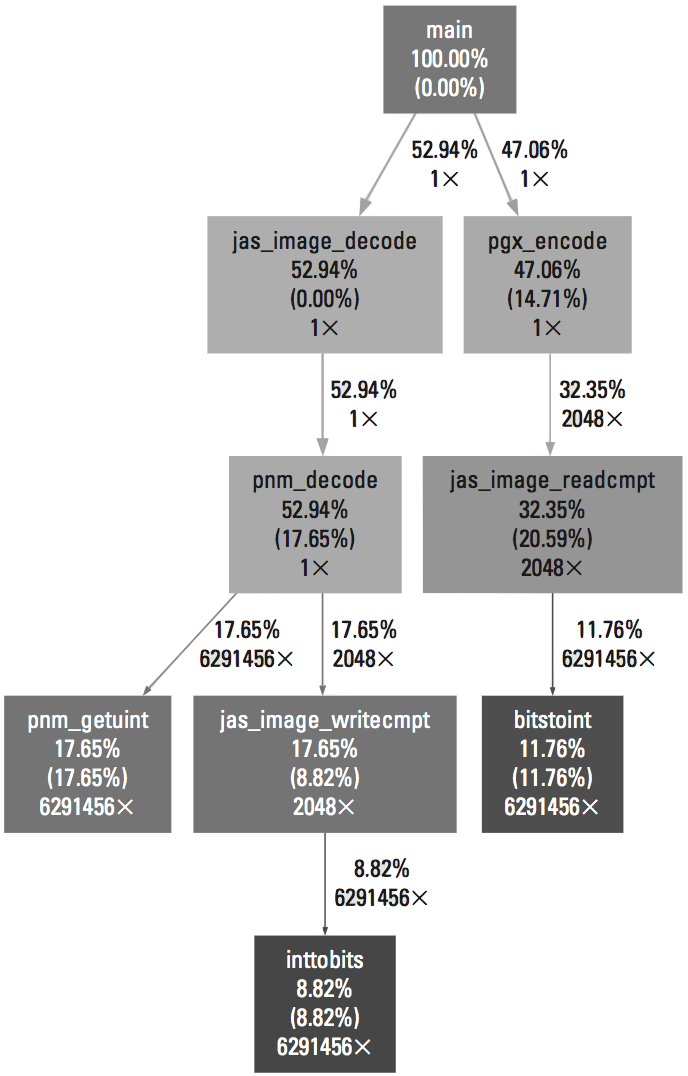
\includegraphics[width=0.8\textwidth]{img/f4-1-2.png}
                  \caption{\Profile\ da codificação de imagem em formato JPEG. Fonte: \cite{Sass2010}.}
               \end{figure}
            \end{column}
            \begin{column}{0.5\textwidth}
               \vspace{-1cm}
               \begin{itemize}
                  \item Procedimento da ferramenta
                  \begin{enumerate}
                     \setlength{\itemsep}{0.8em}
                     \item \textbf{Realiza-se interrupções periódica} no programa; e
                     \item Amostra o seu \textit{program counter}.
                     
                     \item Utiliza-se de um histograma para contar o endereço particular;
                     
                     \item \textbf{Calcula a fração aproximada do tempo} total de execução \textbf{gasto em suas partes}. 
                  \end{enumerate}
               \end{itemize}
            
            \end{column}
         \end{columns}
         \pdfnote{OLHAR OS PARENTESES (\%)}
         \pdfnote{coletar info em tempo de execução.}
         \pdfnote{soft entrada, mensura-se seu tempo.}
         
      \end{frame}


   \subsection{Sistemas Computacionais Wearables}
      %\frame{\centering \bf \Huge \color{beamerCinza} \textit{Sistemas Computacionais \Wearables}}

      \begin{frame}{\Wearables} \vspace{-1em}
         \begin{itemize} \setlength{\itemsep}{1.4em}
            \item Definição
            \begin{itemize} \setlength{\itemsep}{0.4em}
               \item Subconjunto de componentes;
               \item Possibilidade de ter recursos sensoriais e escaneamentos;
               \item Requer serviço autônomo, contínuo, em um longo período de tempo.
               \item Integrar-se ao sistema corporal;
               \item Expandindo suas capacidades;
               \item \textbf{Ou seja, são embutidos inseridos em ambiente \mobile\ de seus usuários, não exercendo a mesma atividade} \cite{Plessl2003}. 
            \end{itemize}
         
            %\item Acesso constante, conveniente, portátil e principalmente \textit{hands-free}.
            
            \item Em 2015, foi previsto um total de 6,5 bi de dispositivos ativamente conectados \cite{RobvanderMeulen2015}
            \begin{itemize} \setlength{\itemsep}{0.4em}
               \item Cerca de 20\% da população possui pelo menos um dispositivo sendo que 10\% utiliza-o todos os dias \cite{lee2016information};
               \item \textbf{Tendência:} Superar dispositivos manuais.
            \end{itemize}
            
         \end{itemize}
         \pdfnote{+ integração entre tecnologia e s.humano}
      \end{frame}  
     
      
      \begin{frame} {\Wearables}{Algumas Definições Científicas} \vspace{-1em}
         % Introdução histórica e geral
         \begin{block}{Segundo \cite{Amorim2017}:} 
            Com a possibilidade de ter um computador acoplado ao corpo, \textbf{proporciona ao usuário um nível de informações} contextualizadas \textbf{dentro de um ambiente interativo}.
         \end{block}
            
            \bigskip
      
         \begin{block}{Segundo \cite{Gemperle1998}:} 
            Dispositivo que possui sua `\textit{wearability}'. Este definido como a \textbf{interação entre o corpo humano e o objeto \textit{wearable} estendendo ao corpo em movimento}.
         \end{block}
      
      \end{frame}
   
      \begin{frame}{\Wearables}{Situação Exemplo} \vspace{-1em}
         \begin{columns}
            \begin{column}{0.6\textwidth}
               \begin{figure}[h] \centering
                  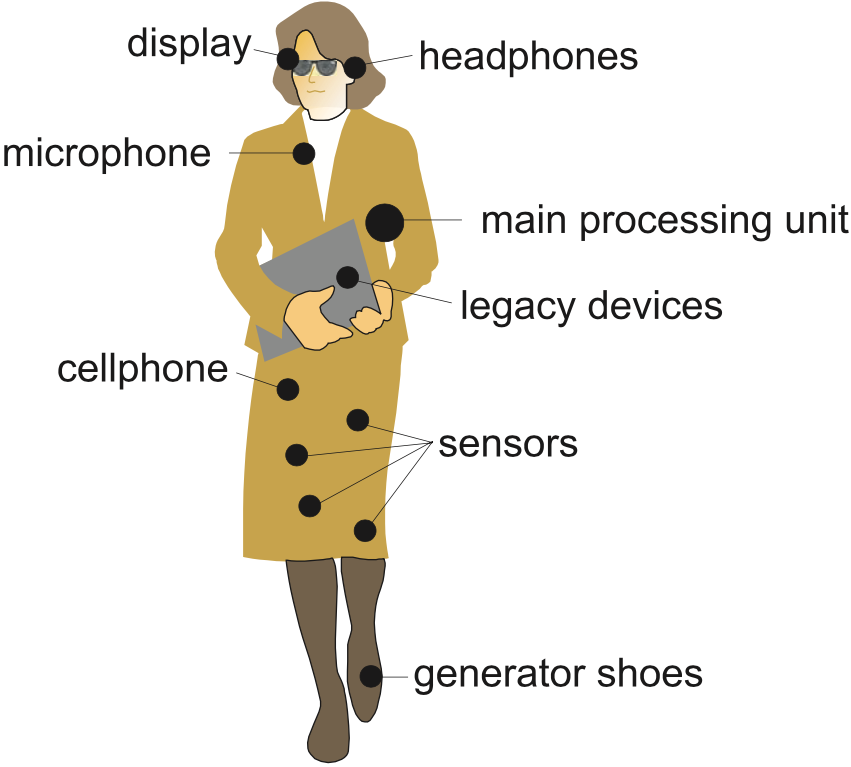
\includegraphics[width=1\textwidth]{img/into-wearable2.png}
                  \caption{Exemplificação de alguns dispositivos \wearables. Fonte: \cite{Plessl2003}.}
                  \label{fig:into-wearable}
               \end{figure}
            \end{column}
            \begin{column}{0.4\textwidth}
               \begin{itemize}
                  \item 
                  Distribuição espacial dos módulos pelo corpo;
                  
                  \item Comunicação:
                  \begin{itemize}
                     \setlength{\itemsep}{1.5em}
                     \item Deve ser avaliada energeticamente \cite{Kymissis1998}.
                     \item \textbf{Pode ser mista, sendo a predominância sem-fio pela mobilidade} \cite{Plessl2003}.
                  \end{itemize}
               \end{itemize}
               
            \end{column}
         \end{columns}
         
      \end{frame}
      
      
         % Característica de um dispositivo wearable
         \begin{frame}{Características de um \Wearable} \vspace{-1em}
            \begin{itemize} \setlength{\itemsep}{1.5em}
               \item Caracteriza-se um \wearable\ acordando \textbf{às suas funcionalidades e requisitos de \hardware}\ \cite{Delabrida2016, Amorim2017}.
               
               \item Sendo essas:
                
               \begin{itemize}
                  \setlength{\itemsep}{0.5em}
                  \item Soluções em \hardware\ \textbf{compartilham uma arq. e org. interna} de recursos comum.
                  
                  \item Também podem ser expandidos às \textbf{características de OS}.
                  
               \end{itemize}
            \end{itemize}
      
            \begin{figure}[h] \centering
               \vspace{-5pt}
               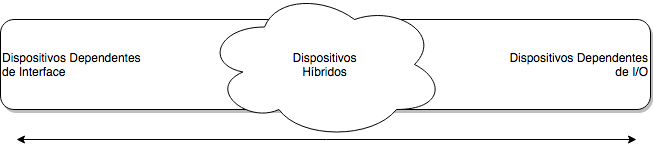
\includegraphics[width=0.9\textwidth]{img/rt-gradiente.png}
               %\vspace{-10pt}
               \caption{Classificação de \wearables. Fonte: Adaptado de \cite{Amorim2017}.}
            \end{figure}
         \end{frame}
      
      \begin{frame}{\Wearable}{Sistemas Operacionais} \vspace{-1em}
            
         \begin{itemize} \setlength{\itemsep}{1.5em}
            \item São comumente \textbf{focado em um único tipo de seguimento} de produto
            \begin{itemize}
               \item Como os \textit{smartwatches}.
            \end{itemize}
            
            \item Vantagens
            \begin{itemize}
               \item Proporcionam aos desenvolvedores um
               \begin{itemize}
                  \item Meio para sua aplicação final; além de
                  \item Produto de alta qualidade.
               \end{itemize}
            \end{itemize}
            
            \item Desvantagens
            \begin{itemize}
               \item Atualmente não existe \textbf{nenhum sistema que satisfaça todos os requisitos} de todas as classificações \cite{Amorim2017}.
            \end{itemize}
         \end{itemize}
      \end{frame}
      
      
      \begin{frame}{\Wearables}{Características a serem Consideradas no \Design} \vspace{-1em}
         
         \begin{itemize}
            \setlength{\itemsep}{0.9em}
            \item \textbf{Performance de multi-nós:} 
            \begin{itemize} \setlength{\itemsep}{0.4em}
               \item \textbf{Tarefas baixa demanda computacional ou nem restrições de tempo rigorosa}: Requer uma performance base fixa;
               
               \item Consideração de restrições de \textbf{tempo-real}.
            \end{itemize}
            
            \item \textbf{Gasto energético consciente:} 
            \begin{itemize} \setlength{\itemsep}{0.4em}
               \item Manter-se ativo e funcional num certo período de tempo;
               \item Gerenciamento do gasto de energia.
               
            \end{itemize}
            
            \item \textbf{Flexibilidade:}
            \begin{itemize} \setlength{\itemsep}{0.4em}
               \item Útil em situações altamente dinâmicas.
               \begin{itemize}
                  \item Pode variar de acordo com as escolhas do usuário ou também com o contexto e local utilizado;
                  \item Trocas de roupa.
               \end{itemize}
               \item Critérios: confiabilidade, disponibilidade e itens dependentes de sua forma como volume e peso.
            \end{itemize}
         \end{itemize}
      \end{frame}
      
      
      \begin{frame}{\Wearable\ + FPGA}{Justificativa  \cite{Plessl2003}} \vspace{-1em}
         \begin{itemize}
            \setlength{\itemsep}{1.6em}
            \item \Wearables\ necessitam
            \begin{itemize}
               \setlength{\itemsep}{0.8em}
               
               \item \textbf{Requisitos de alta performance e consumo de energia consciente:} demandam um sistema computacional econômico;
               
               \item \textbf{Requisitos flexíveis:} demanda um sistema de computação programável de propósito geral.
            \end{itemize}
         
            \item Ao utilizar de um \hardware\ reconfigurável nos permite alcançar
            \begin{itemize}
               \item \textbf{Alto processamento};
               \item \textbf{Com maior eficiência energética} comparando com processadores para computação intensiva em tempo real;
               \item Isso, junto com a disponibilidade de circuito reconfigurável para síntese.
            \end{itemize}
         \end{itemize}
      \end{frame}

%% !TeX encoding = UTF-8
% !TEX root = ../presentation.tex
\section{Trabalhos Relacionados}
   %\frame{\centering \bf \Huge \color{beamerCinza} Particionamento para Sistemas Gerais}
   
   \begin{frame} \vspace{-1em}
      \begin{columns}
         \begin{column}{0.4\textwidth}
            \begin{block}{Definição Introdutória Particionamento \cite{Arato2005}}
               Problema de otimização na qual utiliza-se métodos para auxiliar na decisão de cada componente do \design\ referencial. 
            \end{block}
         \end{column}
         \begin{column}{0.6\textwidth}
            
            \begin{figure}[h] \centering
               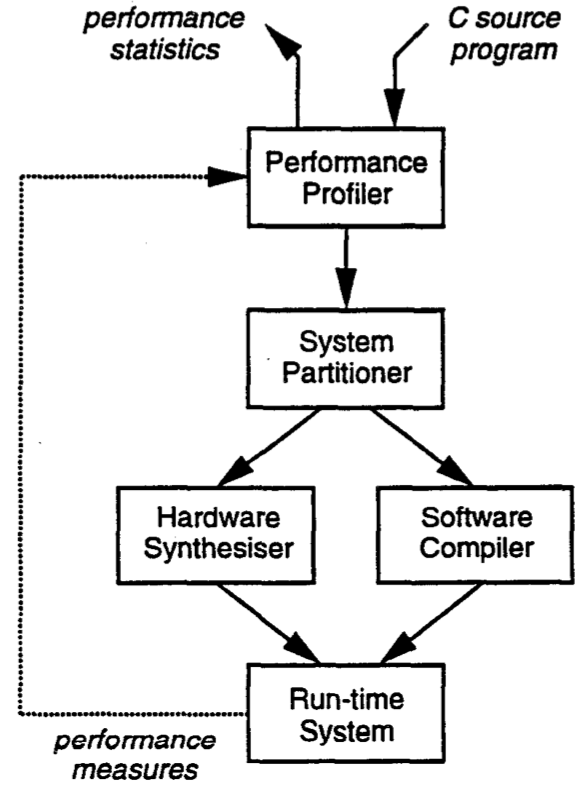
\includegraphics[width=0.8\textwidth]{img/rt-edwards_method.png}
               \caption{Metodologia de \codesign. Fonte: \cite{Edwards1994}.}
               \label{fig:tr-edwards_method}
            \end{figure}
         \end{column}
      \end{columns}   
   
      \pdfinfo{Tanto processos manuais, exatos ou heurísticos.}
   \end{frame}
   
   \begin{frame}{Pioneiro: \cite{Edwards1994}} \vspace{-1em}
      \begin{itemize}
         \setlength{\itemsep}{1.3em}
         \item Utilizam do particionamento para aprimorar a performance do seu \software. 
         \item Realiza-se a tentativa de tratar regiões críticas da aplicação 
         \begin{itemize}
            \item A solução em \software\ não pode chegar à restrições de performance requeridas;
         \end{itemize}
      
         \item Apresenta-se uma metodologia para desenvolvimento \codesign.
         \begin{itemize}
            \setlength{\itemsep}{1.0em}
            \item Consiste na construção do código da aplicação em \textit{C} e sua análise;
            \item Regiões críticas são identificadas e particionadas. 
         \end{itemize}
      
         \item Feito isso, realizar-se mensurações
         \begin{itemize}
            \item  Um novo particionamento é feito.
         \end{itemize}
      
         \item Utiliza-se de um FPGA.
      \end{itemize}
   \end{frame}

   \begin{frame}{Trabalhos com Foco em Otimizações} \vspace{-1em}
      \begin{itemize}
         \setlength{\itemsep}{1.2em}
         \item \cite{Stitt2003} pioneiro no método de otimização \textbf{dinâmico}.
         
         \item Processos:
         \begin{enumerate}
            \setlength{\itemsep}{0.8em}
            \item Detecta a região de mais executada e;
            \item Reimplementa-a em \hardware\ de FPGA.
         \end{enumerate}
      
         \item Afirmam isso vantagens comparado com abordagens tradicionais manuais.
         
         \item Como Stitt, outros propuseram algoritmos \textbf{exatos} baseados em estratégias:
         \begin{itemize}
            \setlength{\itemsep}{0.8em}
            \item \textit{Branch-and-Bound} \cite{Jigang2004, Mann2007, Strachacki2008};
            \item Programação dinâmica \cite{Madsen1997, Wu2006} e;
            \item Programação Linear inteira \cite{Niemann1997}.
         \end{itemize}
      \end{itemize}
   \end{frame}

   \begin{frame}{Trabalhos com Foco em Otimizações} \vspace{-1em}
      \begin{itemize}
         \setlength{\itemsep}{1.8em}
         \item \cite{Nematbakhsh_theeffect} exame da relação entre o \textit{footprint} do FPGA e o \speedup\ do \software.
         \begin{itemize}
            \item FPGA utilizado na implementação de \textit{loops} e sub-rotinas críticas.
         \end{itemize}
      
         \item Abordagem direta utilizando ferramentas comerciais como \textit{Synopys' Nimble Compiler} e \textit{Proceler} para a facilitação do processo.
         
         \item \cite{Yan2017} parte da otimização \textit{position disturbed particle swarm} com otimização invasiva de \textit{weed} como o método de particionamento \hs.
      \end{itemize}
   \end{frame}

   \begin{frame}{\cite{Wang2016}} \vspace{-1em}
      \begin{itemize}
         \setlength{\itemsep}{1.7em}
         \item ``Particionamento depende da exploração de caracterização, estimação e \design\ espacial das métricas de custo e performance sistêmica.''
         \begin{itemize}
            \item Citam o \codesign\ é tão complexo que a simplificação do particionamento só para duas partes não é suficiente para a representação do problema como um todo. 
         \end{itemize}
         
         \item Incluem parâmetros chave de \design\ e uso de recursos que deveriam ser incorporados à modelagem do sistema
         \begin{itemize}
            \item Considera a modelagem de incerteza para particionamento de sistemas com um conjunto melhorado de parâmetros para compartilhamento de recursos \hs.
         \end{itemize}
      
      \end{itemize}
   \end{frame}
   
   \begin{frame}{\cite{Wang2016}} \vspace{-1em}
      \begin{itemize}
         \item Esse terceiro item a ser considerado ao problema de particionamento podem ser definidos em três tipos, sendo esses:
         \begin{enumerate}
            \setlength{\itemsep}{1.5em}
            \item \textbf{Conjunto de recursos necessários para particionar uma dada tarefa:} sendo esses RAM, ROM, DPS, blocos IP do inglês, \textit{intelectual propriety}, entre outros; 
            \item \textbf{Parâmetros de configurações que provê diferentes \textit{trade-off} entre recursos e performances:} exemplo circuitos de multiplicações sintetizados ou não;
            \item \textbf{Dificuldade da mensura de desempenho e impacto no uso de recursos em várias configurações de partição com precisão precisando ter em mente a partição com a natureza incerta\footnote{Teoria da incerteza: Matemática axiomática para modelagem de graus de crença.} dessas estimativas não precisas.}
         \end{enumerate}
      \end{itemize}
   \end{frame}
   \begin{comment}
   
   Como outro trabalho recente que aborda o particionamento, \cite{Choi2016} descreve um \textit{framework} chamado LegUp.
   Com essa ferramenta é possível compilar um \software\ e suas \textit{threads} gerando um sistema \textit{hardware-only} ou também um sistema híbrido particionado paralelo utilizando aceleradores, gerando também todos os itens necessários para tal como memórias sintetizadas e sistemas de interconexões.
   Utilizam duas técnicas de descrição de paralelismo em \software\ sendo elas a \textit{Pthreads} e a \textit{OpenMP} sendo a primeira permite a sintetização de funções operando concorrentemente em \hardware\ com aceleradores, e a segunda usada para gerar os próprios aceleradores executados concorrentemente em um sistema de compartilhamento de memória.
   Afirmam também que a sua ferramenta produz HDL de alta performance que pode ser comparado com circuitos que são gerados por ferramentas HLS comerciais. 
   Os resultados obtidos pelos cientistas \cite{Canis2011} mostraram que a ferramenta consegue gerar produtos tão bons quantos ferramentas HLS comerciais. \todo{olhar}
   
   Entretanto, além de todo arcabouço de algoritmos para escolhas para sistemas de propósito geral tal como os citados, existe ainda uma linha de pesquisa específica do problema na qual trata-se do particionamento em sistemas embutidos.
   \end{comment}
   
  \frame{\centering \bf \Huge \color{beamerCinza} Sistemas Embarcados}   
   
   \begin{frame}{Embarcados} \vspace{-1em}
      \begin{itemize}
         \setlength{\itemsep}{1.8em}
         \item SE é amplamente pesquisado desde 90 \cite{Ernst1993, Gupta1995, Hardt1995, Gajski1994, Bolsens1997}.
         
         \item \cite{Mei2000} Descreve um particionamento além de uma abordagem de escalonamento para DRESs\footnote{Do inglês \textit{dynamically reconfigurable embedded systems}.}
         \begin{itemize}
            \item Para o escalonamento, \cite{Mei2000} Algoritmo Genético.
         \end{itemize}
      
         \item Contribuições
         \begin{itemize}
            \setlength{\itemsep}{1.0em}
            \item Análise de tempo de configuração e;
            \item Análise do tempo de reconfiguração parcial do FPGA.
         \end{itemize}
      
      \end{itemize}
      \pdfnote{Embedded}
      \pdfnote{reconfiguração parcial -> escalonamento p. de alocação restrita.}
   \end{frame}

   \begin{frame}{\cite{Arato2003}} \vspace{-1em}
      \begin{itemize}
         \setlength{\itemsep}{1.8em}
         \item Descreve versões diferentes do particionamento
         \begin{itemize}
            \setlength{\itemsep}{1.0em}
            \item Sistemas de tempo-real e custo restringido respectivamente;
            \item Fornece análise matemática formal do problema, provando que é $ \mathcal{NP} $-difícil.
         \end{itemize} 
      
         \item Utiliza 
         \begin{itemize}
            \setlength{\itemsep}{1.0em}
            \item Programação linear inteira resolvendo de forma otimizada, e;
            \item Outra utilizando GA com soluções próximas ao ótimo global.
         \end{itemize}
      \end{itemize}
   \end{frame}

   \begin{frame}{\cite{Mann2007}} \vspace{-1em}
      \begin{itemize}
         \setlength{\itemsep}{1.2em}
         \item Descrevem uma primeira tentativa para um algoritmo exato, não heurístico, para o problema de particionamento. 
         
         \item Implementa-se a estratégia \textit{branch-and-bound} como um \textit{framework}, permitindo o incremento de outros algoritmos. 
         
         \item Realizaram investigações para incrementar a eficiência do algoritmo com as técnicas:
         \begin{itemize}
            \item \textit{Lower bounds based on LP-relaxation}, uma mecânica de inferência customizada, condições não-triviais necessárias baseadas num algoritmo \textit{minimum-cut}, e diferentes heurísticas com passos pré-otimizados. 
         \end{itemize}
      
         \item Demonstram que podem resolver problemas complexos em tempo razoável. 
         \begin{itemize}
            \item O resultado é em entorno de dez minutos mais rápido que algoritmos exatos anteriores baseados em programação linear inteira para os testes realizados.
         \end{itemize}
      \end{itemize}
      \pdfnote{Prox slide: pesq mais recentes}
   \end{frame}
   
   \begin{frame}{\cite{Hassine2017}} \vspace{-1em}
      \begin{itemize}
         \setlength{\itemsep}{1.5em}
         \item Aplicou otimizações sobre o tempo de execução e gasto energético.
         
         \item O algoritmo proposto destina-se a alcançar um particionamento de grafos à procurar o melhor conjunto da relação energia e tempo de execução.
         
         \item Comparou-se com \textit{Simulated Annealing}, Busca Tabu e Genético
         \begin{itemize}
            \item Mostra-se mais adequado para aplicações em \cores\ de sistemas embarcados que necessitam do equilíbrio no \textit{tradeoff} de sistemas embarcados.
         \end{itemize}
         
      \end{itemize}
   \end{frame}
   
   \begin{frame}{\cite{Trindade2016}} \vspace{-1em}
      \begin{itemize}
         \setlength{\itemsep}{1.8em}
         \item Utiliza do GA para solucionar o problema.
         
         \item Propõe novas abordagens usando técnicas de verificação baseadas nas teorias de módulo de satisfação (SMT, do inglês \textit{satisfiability modulo theories}). 
         
         \item Apresentam um exemplo de particionamento, modelam e solucionam-o usando três diferentes técnicas
         \begin{itemize}
            \setlength{\itemsep}{1.0em}
            \item A ideia principal é aplicar o método de verificação SMT ao particionamento, e;
            \item Comparar os resultados com otimizações tradicionais como ILP e GA.
         \end{itemize}
         
      \end{itemize}
   \end{frame}


   \begin{frame}{\cite{Jozwiak2017}} \vspace{-1em}
      \begin{itemize}
         \setlength{\itemsep}{0.7em}
         \item Seu \textit{survey} considera os aspectos de uma aplicação embutida
         \begin{itemize}
            \item Tecnologias de \design\ com foco sistemas móveis modernos e \wearables.
         \end{itemize}
      
         \item Cita-se dois paradigmas de desen. para SE sobre sistema de multi-processadores heterogêneos. O paradigma de sistemas 
         \begin{itemize} \setlength{\itemsep}{0.5em}
            \item \textbf{\textit{Life-inspired}:} 
            \begin{itemize}
               \item Especifica princípios, características e organização funcional e estrutural de SE com analogia à vida de um organismo inteligente;
               \item Soluções de mecanismos e arquiteturas de sistemas para sua implementação. 
            \end{itemize}
            
            \item \textbf{\textit{Quality-driven}:} 
            \begin{itemize}
               \item Solução para o \design\ de disp. que necessitam de exigências de \textit{real-time}, baixo consumo de energia, entre outros; 
               \item Dessa forma, especifica-se qual a nova qualidade do sistema a ser requeria e como esta meta é obtida. 
               \item ``Define-se \textit{qualidade} de uma solução sistêmica proposta como o \textit{total de sua eficácia}\footnote{Grau em que uma solução atinge seus objetivos.} \textbf{e} \textit{eficiência\footnote{Grau em que uma solução usa recursos para realizar seus objetivos.} na resolução do problema real}''.
            \end{itemize}
         \end{itemize}
      
      \end{itemize}
      \pdfnote{ORIENTADO PELA QUALIDADE}
      \pdfnote{juntas determinam o grau de EXCELÊNCIA}
      
   \end{frame}

   
   \begin{frame}{\cite{Jozwiak2017}} 
      
      \begin{block}{Entretanto, descreveram ao final que \cite{Jozwiak2017}}
         ``Enquanto \designers\ aprenderam bastante na \textbf{construção} de plataformas de \hardware\ heterogêneos altamente paralelos, métodos e ferramentas automatizadas para a sua programação e o paralelismo do algoritmo, bem como o \codesign\ coerente da arquitetura \hs\ \textbf{ainda estão atrasados perante à tecnologia}''.
      \end{block}
   \end{frame}


   \begin{frame}{\Wearable e FPGA}
      \begin{itemize}
         \setlength{\itemsep}{2em}
         \item \cite{Plessl2003, Ahola2007, Abdelhedi2016, Narumi2016, Lee2015} que relacionam FPGAs com aplicação \wearable.
         
         \item Entretanto, nenhum menciona análise metodológica do problema de particionamento \hs\ para \design\ de sistemas computacionais \wearables.
      \end{itemize}
   \end{frame}
% !TeX encoding = UTF-8
% !TEX root = ./presentation.tex
% !TEX spellcheck = pt_BR

\section{Metodologia a ser Executada}
   \subsection{Design\ Referencial de Software\ Utilizando Grafo de Controle de Fluxo}
      \begin{frame}{Design\ de Sistemas Embutidos}
         \begin{itemize}  \setlength{\itemsep}{1.6em}
            \item Fundamentos para o compreendimento do particionamento;
            \item Metodologia baseada em \parencite{Sass2010, Arato2003, Arato2005, Mann2007, Hassine2017}.
         \end{itemize}
      \end{frame}
   
      \begin{frame}{Grafo de Controle de Fluxo (GCF)} \vspace{-1em}
         \begin{itemize}
            \setlength{\itemsep}{1.5em}
            \item Por que utilizá-lo:
            \begin{itemize}
                \setlength{\itemsep}{0.5em}
               \item \textbf{Descreve um sistema}, tanto em \software\ ou \hardware, \textbf{livre de uma especificação de forma};
               \item Rápidos protótipos, referenciado como \design\ de referência de \software\ (DRS).
            \end{itemize}
   
            \item O sistema inicial é dado como \textbf{grafo de tarefas/rotinas}, define-se \bx{$ C = (B, F) $} onde
            \begin{description}
               \item [$B$:] vértices que representam os blocos básicos; e 
               \item [$F$:] arestas que indicam a todas as possibilidades de caminhos entre os blocos.
            \end{description}
         \end{itemize}
      \end{frame}
   
      \begin{frame} %\vspace{-1em}
         \begin{figure}[h] \centering
            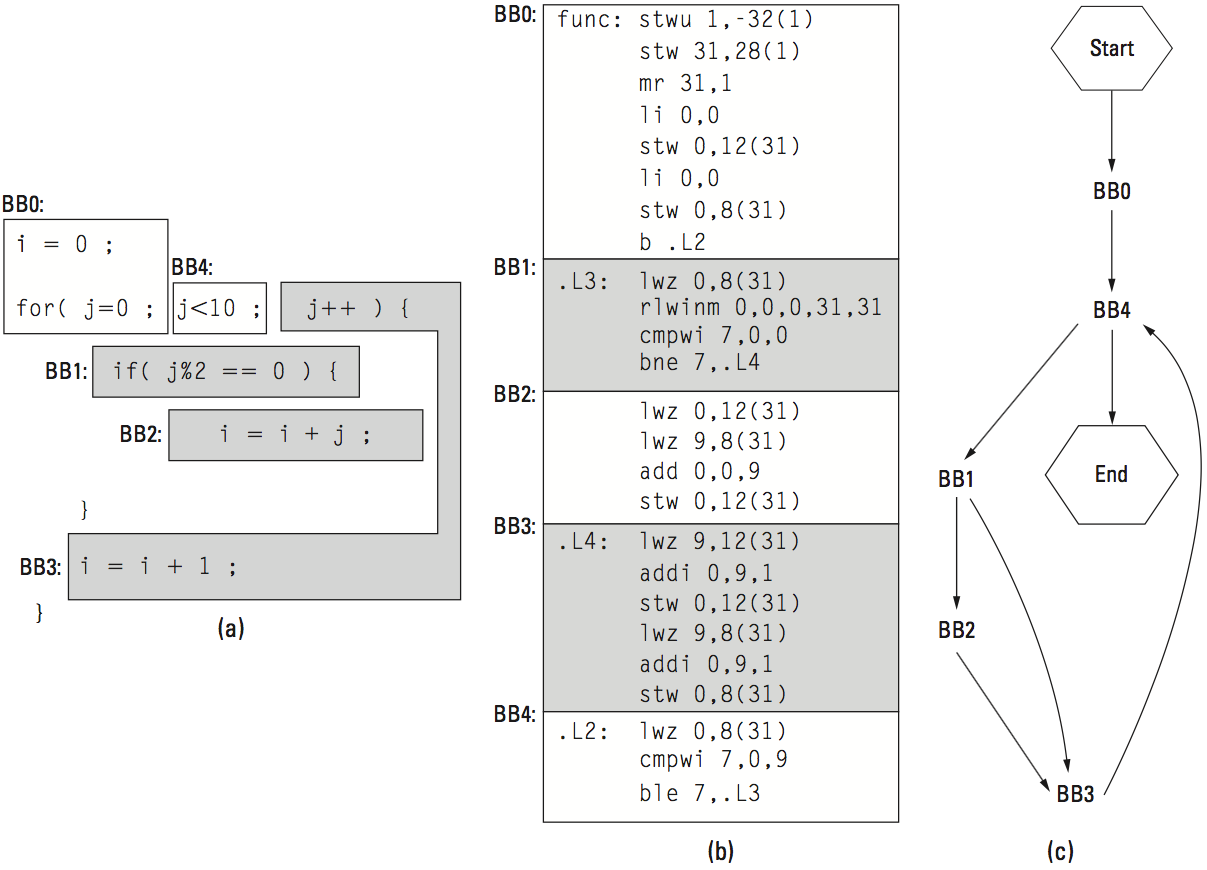
\includegraphics[width=0.89\textwidth]{img/f3-6.png}
            \caption{Identificação de blocos básicos e a representação de cada modelo de descrição de \software.}
            %\label{fig:f3-6}
         \end{figure}
      \end{frame}
   
   \subsubsection{Grafo de Chamada (GC)}
   
      \begin{frame}{Grafo de Chamada (GC)}
         %Modelado uma sub-rotina de um DRS utilizando o GCF, define-se o Grafo de Chamada (GC).
   
         \begin{itemize}
            \setlength{\itemsep}{0.6em}
            \item \textbf{Consiste num conjunto de Grafos de Controle de Fluxo}, um por sub-rotinas, ou seja
               \bx{$\mathcal{C} = {C_0, C_1, \dots C_{n-1}}$}
            onde 
            \begin{description}
               \item[$ C_i = (B_i, F_i) $:] \textbf{representa o GCF de uma sub-rotina} $ i $.
            \end{description}
   
            \item Grafo estático de chamada da aplicação é \bx{$\mathcal{A} = (\mathcal{C}, \mathcal{L}) \label{eq:a}$} onde
            \begin{description}
               \item [\A:] representa uma aplicação específica; e
               \item [$ \mathcal{L} \subseteq \mathcal{C} \times \mathcal{C} $:] plano cartesiano das invocações de rotinas.
            \end{description}
   
         \end{itemize}
   
         \begin{block}{Duas sub-rotinas são relacionadas se}
            Podem ser determinadas, no tempo de compilação, que a \textbf{sub-rotina $ i $ tem potencial de invocar a sub-rotina $ j $}, ou seja, \bx{$ (C_i, C_j) \in \mathcal{L} $}.
         \end{block}
         \pdfnote{Para entendimento da partição}
         \pdfnote{um subconjunto do plano cartesiano dos GCF}
      \end{frame}
   
    \begin{frame}{Definição Formal de Partição}
        Uma partição com $n$ partição $ \mathcal{S} = \{S_0, S_1, \dots, S_n\} $ de um conjunto universal $ U $ \textbf{é um conjunto de subconjuntos de} $ U $ sendo que
        %
        \begin{eqnarray}
        \bigcup_{S \in \mathcal{S}} S &=& U \\ \pause
        \forall S, S' \in \mathcal{S} | S \cap S' &=& \emptyset \\
        \forall S \in \mathcal{S}\ |\ S &\neq& \emptyset
        \end{eqnarray}
        \pause
        Considere $ U = \{a, e, i, o, u, y\} $. Uma partição $ \mathcal{X}_i $ de $ U $:
        \begin{eqnarray}
        \mathcal{X}_a &=& \left\{\{a, e, i, o, u\}, \{y\}\right\} \label{eq:xa} \\
        \mathcal{X}_b &=& \left\{\{a\}, \{e\}, \{i\}, \{o\}, \{u\}, \{y\}\right\} \label{eq:part_a} \\
        \mathcal{X}_c &=& \left\{\{a\}, \{e\}, \{i\}, \{o\} \right\} \label{eq:part_c} \\
        \mathcal{X}_d &=& \left\{\{a, e, i\}, \{i, o, u, y\}, \{\}\right\} \label{eq:part_d}
        \end{eqnarray}
        
        \textit{$\mathcal{X}_c$ viola a Eq. 1, $\mathcal{X}_d$ viola Eqs. 2 e 3.}
        
        \pdfnote{1: cada ele d $ U $ é membro de 1+ $ S \in \mathcal{S} $}
        \pdfnote{2,3: S são emparelhados disjuntos e não vazio}
        \pdfnote{cada ele $ U $ termina em um dos $\mathcal{S}$ e nenhum dos s é vazios.}
    \end{frame}
   
   
   
   \subsection{Particionamento}
      \begin{frame}{Aplicar o Formalismo à Aplicação $\mathcal{A} = (\mathcal{C}, \mathcal{L})$}
         \begin{itemize}
            \item Assume-se que
            \begin{description}
               \item [Universo:] é o conjunto dos \textit{blocos básicos} $B$ de todas as sub-rotinas de um dispositivo \wearable;
               
               \item [$\therefore U$:] é as partições de sub-rotinas
            \end{description}
            
            %
            \begin{equation}
               U = \bigcup_{C \in \mathcal{C}} B(C) \label{eq:bigcup}
            \end{equation}
            ou seja, uma partição $\mathcal{S}$
            \begin{equation}
               \mathcal{S}  = \left \{
               \underbrace{\left \{ b_0, b_1, \dots, b_i \right \}}_{\text{sub-rotina }C_0},
               \underbrace{\left \{ b_i, b_{i+1}, \dots, \right \}}_{\text{sub-rotina }C_1},\dots
               \underbrace{\left \{ b_j, b_{j+1}, \dots, \right \}}_{\text{sub-rotina }C_{n-1}}
               \right \}
            \end{equation}
   
            \item Propósito
            \begin{enumerate}
               \item \textbf{Reorganizar a partição} de blocos básicos e então;
               \item \textbf{Mapear} cada subconjunto.
            \end{enumerate}
   
         \end{itemize}
      \end{frame}
   
   
   
      \begin{frame}{Aplicar o Formalismo à Aplicação $\mathcal{A} = (\mathcal{C}, \mathcal{L})$}
         \begin{itemize}  \setlength{\itemsep}{0.6em}
            \item Dessa forma pode-se
            \begin{itemize}
               \item Criar e remover subconjuntos \textbf{não vazios};
               \item Mover blocos básicos ao redor até ter uma nova partição.
            \end{itemize}
   
            \item $\therefore \mathcal{A}’ = (\mathcal{C}’, \mathcal{L}’) $, inferido a partir da reorganização da partição $ \mathcal{X}’ $.
   
               \bigskip
   
            \item Em seguida, mapeia-se cada subconjunto de $ \mathcal{X} $ para ambos \hs
   
         \end{itemize}
            { \footnotesize
            \begin{equation}
               \mathcal{X}'   = \left \{
               \underbrace{
                  \underbrace{
                     \left \{ b_j, b_{j+1}, \dots, \right \}
                  }_{\text{sub-rotina }C_k}
                  \underbrace{
                     \left \{ b_k, b_{k+1}, \dots, \right \}
                  }_{\text{sub-rotina }C_l}
                  \dots
               }_{\text{\software}}
               \
               \underbrace{
                  \underbrace{
                     \left \{ b_0, b_1, \dots, b_i \right \}
                  }_{\text{sub-rotina }C_r}
                  \underbrace{
                     \left \{ b_i, b_{i+1}, \dots, \right \}
                  }_{\text{sub-rotina }C_s}
                  \dots
               }_{\text{\hardware}}
               \right \} \label{eq:part_final}
            \end{equation}
            }
      \end{frame}
   
   
   
   \subsection{Ganho de Performance}
   
      \begin{frame}{Ganho de Performance} \vspace{-1em}
         \begin{itemize} \setlength{\itemsep}{1.0em}
            \item \textbf{\Software:} Análise de ordem de complexidade;
            \item \textbf{\Hardware:} Não possui um guia geral para comparação, e por isso utiliza-se ganho de performance.
   
            \item Definições prévias
            \begin{description} \setlength{\itemsep}{0.4em}
               \item [$ s(i) $:] tempo de execução esperado para uma invocação de uma sub-rotina $ i $;
               \item [$ h(i) $:] tempo de execução em \hardware;
               \item [$ m(i) | i \in \mathcal{H} $:] aproximação do montante gasto na transferência de um estado ou o custo de configuração e latência;
               \item [$ \gamma $:] representa o ganho de performance (speedup), $ \gamma > 1.0 $.
            \end{description}
         \end{itemize}
      
         \begin{equation}
            \gamma(i) = \frac{s(i)}{h(i) + m(i)}
         \end{equation}
      \pdfnote{y = gamma}
      \end{frame}
   
   
      \begin{frame}{Ganho de Performance} \vspace{-1em}
         \begin{block}{Do que a aplicação depende para ter maior velocidade?}
            \textbf{Ganhos de performance do recurso} e o \textbf{quão frequentemente ele é utilizado} no \design\ referencial de \software.
         \end{block}
      
         \begin{itemize}
            \item \textbf{Fração do tempo de um recurso em \software}\ $ p(i) $ a partir de informações de \textit{profile}.
         \end{itemize}
            \vspace{-1em}
         \begin{eqnarray}
            %\gamma(i) & = & \frac{s(i)}{h(i) + m(i)} \\
            \Gamma & = & \left [
                                 (1 - p(i))
                                 +
                                 \frac{
                                    p(i)
                                 }{
                                    \gamma(i)
                                 } \right 
                              ]^{-1} \\
%            \Gamma & = & \left [
%                                 (1 - p(i))
%                                 +
%                                 \frac{
%                                    p(i)
%                                 }{
%                                    \frac{s(i)}{h(i) + m(i)}
%                                 } \right 
%                                 ]^{-1}
\Gamma (\mathbb{D}) & = &
\left [
1 + \sum _{i \in \mathbb{D}} \left (
\frac{
   p(i)
}{
   \gamma(i)
}-p(i)
\right)
\right ]^{-1}
         \end{eqnarray}
         
         \begin{description}
            \item [$\gamma(i)$:] performance individual de cada recurso (acelerador);
            \item [$p(i)$:] fração de tempo de um recurso particular (\software);
            \item [$\mathbb{D}$:] recursos em \hardware.
         \end{description}
         
         \pdfnote{Inversao: da taxa de execução p tempo de execução, mantendo o sentido de GanPerf.}
      
      \end{frame}
   
      \begin{frame}{Consideração de Recursos}
         \begin{itemize}
            \item Contar-se o número de células lógicas requeridas para cada recurso
         \end{itemize}
         \begin{description}
            \item [$ r_{FPGA} $:] total de números de células lógicas \textbf{disponíveis};
            
            \item [$ r(i) $:] quantidade de células lógicas \textbf{por cada recurso} $ i $.
         \end{description}
            
            \begin{eqnarray}
            \sum_{i \in \mathbb{D}} r(i) < r_{FPGA} & \quad \text{e} \quad & 
            \vec{r}_{FPGA} =
            \begin{pmatrix}
            r_{Logic\ Cells} \\
            r_{Memory}\\
            r_{DSP}\\
            \vdots \\
            r_{n-1}
            \end{pmatrix}
            \end{eqnarray}
            
            \begin{equation}
            \therefore \sum_{i \in \mathbb{D}} \vec{r}(i) < \vec{r}_{FPGA}
            \end{equation}
            
         \pdfnote{Implementar tudo em h ignorando custos de desenvolvimento/recursos.}
         \pdfnote{D é o conjunto de recurso no \design.}
         \pdfnote{rotas não sao calculadas}
      \end{frame}
      
      
   \subsection{A Proposta: Particionamento para Sistemas Wearable}

      \begin{frame}{Formulação do Problema para \Wearables}
         \begin{itemize}
            \item Definições
            \begin{description}
               \item [$ \mathbb{D} $:] todos os recursos em \hardware;
               \item [$ \mathbb{C} $:] conjunto candidatos;
            \end{description}
         
            \begin{equation}
            \begin{array}{rrcl}
            \text{max}                 & \Gamma ( \mathbb{D})               & ~   & ~                \\
            & & & \\
            subject\ to & \sum_{i \in \mathbb{D}} \vec{r}(i) & < & \vec{r}_{FPGA}
            \end{array}
            \label{eq:constraints}
            \end{equation}
            
               \bigskip
            
            \item Ou seja
      
            \begin{enumerate} \setlength{\itemsep}{0.6em}
               \item Encontrar todas as partições de $ U $;
               \item Sintetizá-las;
               \item \textit{Profiling};
               \item Avaliar quantitativamente cada $ \Gamma $.
            \end{enumerate}
         \end{itemize}
      \pdfnote{p gamma}
      \end{frame}
   
      \begin{frame}[fragile]
         \begin{figure}
            \begin{tikzpicture}[auto, node distance=2.5 cm, >=latex']
            %\tikzstyle{block}    = [draw, rectangle, minimum height=2em, minimum width=4em, fill=red!20]
            %\tikzstyle{input}    = [coordenate]
            %\tikzstyle{output}   = [coordenate]
            %\tikzstyle{pinstyle} = [pin edge={to-,thin,black}]
            \matrix[column sep = .75cm, row sep = .375cm]{
               & \node[draw, shape=rectangle, fill=red!20, visible on=<1->] (hl) {High Level Source}; & \\
               & \node[draw, shape=rectangle, fill=red!20, visible on=<2->] (profile)    {Profiling}; & \\
               & \node[draw, shape=rectangle, fill=red!20, visible on=<3->] (candidate) {Gets Candidates};& \\
               \node[draw, shape=rectangle, fill=red!20, visible on=<4->] (soft) {Software Compiler}; & & 
               \node[draw, shape=rectangle, fill=red!20, visible on=<4->] (hard) {Hardware Synth}; \\
               & \node[draw, shape=rectangle, fill=red!20, visible on=<5->] (evaluate) {Evaluates it};  & \\
               & \node[draw, shape=rectangle, fill=red!20, visible on=<6->] (solve) {Solved};  & \\
            }; 
            \draw [->, thick, visible on=<1->] (hl) -- (profile);
            \draw [->, thick, visible on=<2->] (profile) -- (candidate);
            \draw [->, thick, visible on=<3->] (candidate) -- node {Non Candidates} (soft) ;
            \draw [->, thick, visible on=<3->] (candidate) -- node {Candidates} (hard) ;
            \draw [->, thick, visible on=<4->] (soft) -- (evaluate);
            \draw [->, thick, visible on=<4->] (hard) -- (evaluate);
            \draw [->, thick, visible on=<5->] (evaluate) -- (solve) ;
            \end{tikzpicture}
            \caption{Fluxo de execução do Particionamento.}
         \end{figure}
      \end{frame}
   
   
   \begin{frame}[fragile]
      \begin{figure}
         \begin{tikzpicture}[auto, node distance=2.5 cm, >=latex']
         \matrix[column sep = .75cm, row sep = .375cm]{
            \node[draw, shape=rectangle, fill=red!20, visible on=<1->] (fs1) {Function 1};
            & & \\
            \node[draw, shape=rectangle, fill=red!20, visible on=<1->] (fs2) {Function 2};
            & & \\
            \node[draw, shape=rectangle, fill=red!20, visible on=<1->] (fs3) {Function 3};
            & & \\
            \node[draw, shape=rectangle, fill=red!20, visible on=<1->] (fs4) {Function 4};
            & & \\
            \node[draw, shape=rectangle, fill=red!20, visible on=<1>] (fs51) {Function 5};
            \node[draw, shape=rectangle, fill=red!20, visible on=<2>] (fs52) {\textit{Function 5}};
            \node[draw, shape=rectangle, fill=red!20, visible on=<3->] (fs53) {Invocation 5};
            & & 
            \node[draw, shape=rectangle, fill=red!20, visible on=<2->] (fh5) {Function 5};
            \\
            \node[draw, shape=rectangle, fill=red!20, visible on=<1->] (fs6) {Function 6};
            & & \\
            \node[draw, shape=rectangle, fill=red!20, visible on=<1->] (fs7) {Function 7};
            & & \\
         }; 
         \node[coordinate, xshift=1.5cm,  yshift=0.5cm]  (nAux1) at (fs1) {};
         \node[coordinate, xshift=-1.5cm, yshift=-1cm] (nAux2) at (fs7) {};
         \draw [dashed] (nAux1) -| (nAux2) -| (nAux1) node [above, pos=0.38] {Software};
         
         \node[coordinate, xshift=1.5cm,  yshift=4.2cm]  (nAux1) at (fh5) {};
         \node[coordinate, xshift=-1.5cm, yshift=-2.9cm] (nAux2) at (fh5) {};
         \draw [dashed] (nAux1) -| (nAux2) -| (nAux1) node [above, pos=0.38] {Hardware};
         
         \draw [->, thick, visible on=<2>] (fs52) -- (fh5);
         \draw [<->, thick, visible on=<3>] (fs53) -- (fh5);
         
         %\draw [->, thick, visible on=<2->] (profile) -- (candidate);
         %\draw [->, thick, visible on=<3->] (candidate) -- node {Non Candidates} (soft) ;
         %\draw [->, thick, visible on=<3->] (candidate) -- node {Candidates} (hard) ;
         %\draw [->, thick, visible on=<4->] (soft) -- (evaluate);
         %\draw [->, thick, visible on=<4->] (hard) -- (evaluate);
         %\draw [->, thick, visible on=<5->] (evaluate) -- (solve) ;
         \end{tikzpicture}
         \caption{Particionamento de uma visão geral.}
      \end{figure}
\end{frame}
      
   \begin{comment}
      
   \subsection{Proposta de Procedimento Analítico}
      \begin{frame}{Procedimento Analítico Proposto}
         \scalebox{.78}{  
            \begin{algorithm}[H]
               \SetKwData{itt}{it}
               \SetKwData{pl}{partition\_list}
               \SetKwData{complexSet}{how\_complex\_set\_is}
               \SetKwData{md}{matriz\_dados}
               \SetKwData{complexSet}{how\_complex\_set\_is}
               \SetKwFunction{graph}{makes\_graph}
               \SetKwFunction{porte}{analyses\_complex\_set}
               \SetKwFunction{synth}{synthesizes}
               \SetKwFunction{resources}{resources\_used}
               \SetKwFunction{die}{die\_used}
               \SetKwFunction{energy}{energy\_spent}
               \SetKwFunction{profiling}{profile}
               \SetKwFunction{performance}{performance\_analysis}
               \SetKwFunction{factor}{complexity\_factor}
               \SetKwFunction{ilp}{integer\_linear\_solve}
               \SetKwFunction{heuristic}{heuristic}
               
               %\BlankLine
               \Begin{
                  
                  \BlankLine
                  \profiling{}\;
                  \BlankLine
                  
                  \tcp{extration project analyses}
                  \graph{Flow Control Graph}\;
                  \graph{Call Graph}\;
                  %\complexSet $\leftarrow$ \porte{}\tcp*{verify if it is a big project}
                  
                  \BlankLine
                  
                  \If{exist partitions that can be synthesized}{
                     \ForEach{partition project:\itt $\in$ \pl}{
                        \synth{\itt}\;
                        \BlankLine
                        \resources{\itt}\tcp*{analysis after synth}
                        \die{\itt}\;
                        \energy{\itt}\;
                        %\BlankLine
                        
                        
                        \performance{\itt}\;
                     }
                     \BlankLine
                     
                     %\uIf(\tcp*[f]{verify if it is a small project}){\factor{\complexSet}}{
                     \ilp{\pl}\tcp*{analyse quantitatively each $ \Gamma $}
                     %}
                     %\lElse{
                     %\heuristic{\pl}\;
                     %}
                  }
               }
               \caption{Metodologia para avaliação de wearables.}
            \end{algorithm}
         }
      \end{frame}
   \end{comment}
%% !TeX encoding = UTF-8
% !TEX root = ./presentation.tex

   \begin{frame}{\Wearable: Capacete para Segurança de Ciclistas}{Leitura de Sensores}
      \scalebox{.7}{
         \begin{algorithm}[H]
             \SetKwData{data}{datas}
             \SetKwData{typew}{type\_warning}
             \SetKwData{sx}{sensor$_i$}
             \SetKwFunction{leSensores}{read\_sensors}
             \SetKwFunction{preprocess}{pre\_process}
             \SetKwFunction{process}{process}
             \SetKwFunction{atuacao}{operate}
             \SetKwFunction{finterrupt}{do\_interruption}
             \SetKwFunction{bu}{backup}
             \SetKwFunction{leds}{do\_leds\_warning}
             \SetKwData{btypew}{buffer\_type\_warning}
             
             \BlankLine
             \KwIn{sensors reads.}
             \KwOut{backups and interruptions signals.}
             \BlankLine
             
             \Begin{
                 \tcp{statements}
                 \sx\tcp*{$i$ information's source}
                 \data\tcp*{data's matrix before handling}
                 \typew\tcp*{type of warning to do to user}
                 \BlankLine
                 
                 \While{wearable mode on}{
                     \data $\leftarrow$ \leSensores{\sx}\;
                     \BlankLine
                     
                     \tcp{process the datas}
                     \typew $\leftarrow$ \process{\data}\;
                     
                     \BlankLine
                     \If{\typew $=$ dangerous}{
                         \finterrupt{\typew}\;
                         \leds{\btypew}\;
                     }                  
                     
                     \BlankLine
                     \bu{\data}\;
                 }
                 \BlankLine
             }
             
             \caption{Wearable 2 - Procedimento que realiza leituras de sensores e armazena seus dados em memória não-volátil.}
             \label{alg:wearable2_leituras}
         \end{algorithm}
      }
\end{frame}

   
   \begin{frame}{Procedimento Analítico Proposto}
      \scalebox{.78}{  
         \begin{algorithm}[H]
            \SetKwData{itt}{it}
            \SetKwData{pl}{partition\_list}
            \SetKwData{complexSet}{how\_complex\_set\_is}
            \SetKwData{md}{matriz\_dados}
            \SetKwData{complexSet}{how\_complex\_set\_is}
            \SetKwFunction{graph}{make\_graph}
            \SetKwFunction{porte}{analyse\_complex\_set}
            \SetKwFunction{synth}{synthesize}
            \SetKwFunction{resources}{resource\_used}
            \SetKwFunction{die}{die\_used}
            \SetKwFunction{energy}{energy\_spent}
            \SetKwFunction{profiling}{profile}
            \SetKwFunction{performance}{performance\_analysis}
            \SetKwFunction{factor}{complexity\_factor}
            \SetKwFunction{ilp}{integer\_linear\_solve}
            \SetKwFunction{heuristic}{heuristic}
            
            %\BlankLine
            \Begin{
               
               \BlankLine
               \profiling{}\;
               \BlankLine
               
               \tcp{extration project analyses}
               \graph{Flow Control Graph}\;
               \graph{Call Graph}\;
               %\complexSet $\leftarrow$ \porte{}\tcp*{verify if it is a big project}
               
               \BlankLine
               
               \If{exist partitions that can be synthesized}{
                  \ForEach{partition project:\itt $\in$ \pl}{
                     \synth{\itt}\;
                     \BlankLine
                     \resources{\itt}\tcp*{analysis after synth}
                     \die{\itt}\;
                     \energy{\itt}\;
                     %\BlankLine
                     
                     
                     \performance{\itt}\;
                  }
                  \BlankLine
                  
                  %\uIf(\tcp*[f]{verify if it is a small project}){\factor{\complexSet}}{
                  \ilp{\pl}\tcp*{analyse quantitatively each $ \Gamma $}
                  %}
                  %\lElse{
                  %\heuristic{\pl}\;
                  %}
               }
            }
            \caption{Metodologia para avaliação de wearables.}
         \end{algorithm}
      }
   \end{frame}

   \begin{frame}{\Wearable: Capacete para Segurança de Ciclistas}
        \vspace{-0.8em}
      
      \begin{figure}[h] \centering
         \includegraphics[width=0.67\textwidth]{img/capacete.png}
         \vspace{-1em}
         \caption{Grafo do projeto Wearable.}
      \end{figure}
      
   \end{frame}

    \begin{frame}{\Wearable: Capacete para Segurança de Ciclistas}
    \vspace{-0.8em}
    
        \begin{figure}[h] \centering
        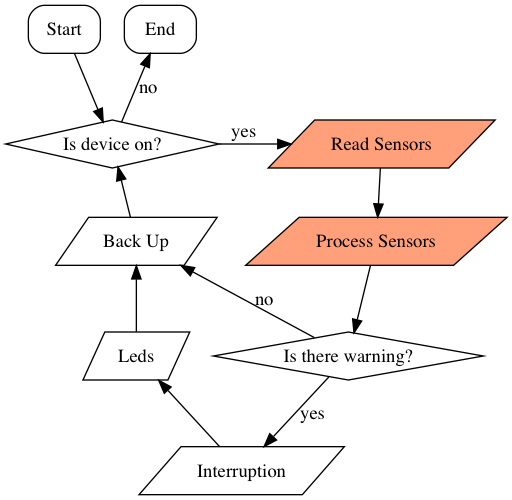
\includegraphics[width=0.67\textwidth]{img/capacete2.png}
        \vspace{-1em}
        \caption{Grafo do projeto Wearable.}
        \end{figure}
    \end{frame}


    \begin{frame}{\Wearable: Capacete para Segurança de Ciclistas}
        \vspace{-0.8em}
        
        \begin{columns}
            \begin{column}{0.6\textwidth}
                
                \begin{figure}[h] \centering
                    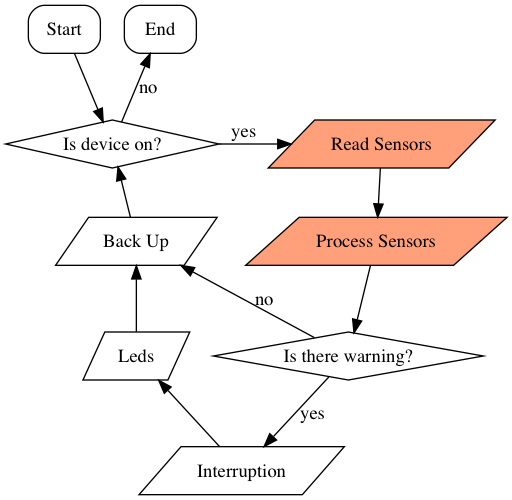
\includegraphics[width=1\textwidth]{img/capacete2.png}
                    \vspace{-1em}
                    \caption{Grafo do projeto Wearable.}
                \end{figure}
            \end{column}
            \begin{column}{0.4\textwidth}
                \vspace{-1cm}
                \begin{itemize}
                    \setlength{\itemsep}{1.4em}
                    \item Análise de $1..3$ sensores
                    \begin{enumerate}
                        \setlength{\itemsep}{0.8em}
                        \item Ao utilizar vários sensores, tem-se um \textbf{espaço}.
                    \end{enumerate}
                    \item Funções com complexidade diferentes
                    \begin{itemize}
                        \item Testar a aplicação utilizando $\mathcal{O}(1)$, $\mathcal{O}(n\log n)$ e $\mathcal{O}(n^2)$.
                    \end{itemize}
                \end{itemize}
                
            \end{column}
        \end{columns}
    \end{frame}

%% !TeX encoding = UTF-8
% !TEX root = ./presentation.tex
\section{Conclusões Parciais e Trabalho Futuro}
   \subsection{Considerações Finais}
   \begin{frame}{Conclusões Parciais} \vspace{-1em}
      \begin{itemize} \setlength{\itemsep}{1.4em}
         \item 
         %demora da pesquisa em wearables
         Mesmo a \textbf{tecnologia embarcada evoluindo} nos mais diversos fins
         \begin{itemize}
            \item \Wearables\ tiveram seu primeiro aparecimento em em 1996 por Mann \cite{Mann1996}.
         \end{itemize}
      
         \item Motivos desse atraso
         \begin{itemize} \setlength{\itemsep}{0.4em}
            \item \textbf{Necessidade da miniaturização};
            \item \textbf{Mobilidade}; e
            \item \textbf{Eficiência energética}.
         \end{itemize}
         
         %não tem particionamento para wearables
         \item Há várias pesquisas relacionadas à área de embarcados no âmbito de particionamento de \hs
         \begin{itemize}
            \item Inclusive com FPGAs.
         \end{itemize}
         
      \end{itemize}
   \end{frame}

   \begin{frame}{Objetivos Realizados e Trabalho Futuro} \vspace{-1em}
      \begin{itemize} \setlength{\itemsep}{0.8em}
         
         % objetivos concluídos até então
         \item \textbf{Objetivos realizados}
         \begin{itemize}
            \item Apresentação do problema de particionamento com foco em sistemas \wearables;
            
            \item Apresentação de:
            \begin{itemize}
               \item \textbf{Soluções utilizadas atualmente};
               \item \textbf{Ferramentas HLS como LegUp e OpenCL} para a geração de aceleradores.
            \end{itemize}
            
            \item \textbf{Metodologia} a ser utilizada.
         \end{itemize}
         
         \item \textbf{Próximos passos}
         \begin{itemize}
            
            \item \textbf{Geração de HDL}
            \begin{itemize}
               \item LegUp;
               \item OpenCL.
            \end{itemize}
            
            \item \textbf{Testes}
            \begin{itemize}
               \item Totalmente em nível de \software;
               \item Híbridos.
            \end{itemize}
            
            \item \textbf{Propósito:} Com a utilização de recursos do FPGA %Wolf1994
            \begin{itemize}
               \item Redução do tempo de seu desenvolvimento até a disposição do produto ao mercado.
            \end{itemize}
         \end{itemize}
      \end{itemize}
   \end{frame}


\frame{\titlepage}

\appendix

\section*{Bibliografia}

\begin{frame}[allowframebreaks]
   \frametitle{Referências}
   %\printbibliography
   %\bibliographystyle{plain}
   \printbibliography
   
   
   %\bibliographystyle{amsalpha}
   %\bibliography{bibliography}
\end{frame}

\maketitle

% !TeX encoding = UTF-8
% !TEX root = ./presentation.tex
\section{HLS}

\section{FPGA}
   
   \begin{frame}{Tecnologia dos FPGA} \vspace{-1em}
      \textbf{Vários módulos lógicos programáveis} relativamente \textbf{pequenos} e independentes, interconectados.
      
      \begin{itemize}
         \item A maioria dos FPGAs utilizam \textit{look-up table} (LUT) para criar as funções lógicas desejadas.
         \begin{itemize} 
            \setlength{\itemsep}{1.5em}
            \item Uma LUT funciona como uma tabela-verdade, ou seja, registradores programáveis. 
            \item Cada módulo lida com até quatro ou cinco variáveis de entrada;
            \item A saída é programada para criar a função combinacional armazenando valores verdadeiros e falsos adequado a cada combinação de entrada;
            \item Eles não são associados a nenhum pino de entrada e saída (I/O, do inglês \textit{Input and Output}). 
         \end{itemize}
         
      \end{itemize}
      \pdfnote{pequenos pra criar funções +}
   \end{frame}
   
   
   \begin{frame}{Tecnologia dos FPGA} \vspace{-1em}
      Vários módulos lógicos programáveis relativamente \textbf{pequenos} e \textbf{independentes}, \textbf{interconectados}.
      
      \begin{itemize}
      \setlength{\itemsep}{1.2em}
      
      \item Os recursos de roteamento de sinal programável dentro do chip
      \begin{itemize}
         \item Os atrasos de sinal em um projeto dependem do roteamento real de sinal selecionado pelo \software\ de programação. 
      \end{itemize}
      
      \item Pinos de I/O são conectados ao bloco programável de entrada e saída que, por sua vez, é conectado aos módulos lógicos com linhas de roteamento selecionadas.
      \bigskip
      \item Assim, FPGAs são chips que podem ser programados instantaneamente para funções de qualquer circuito digital \cite{Choi2016}.   
      \end{itemize}
      \pdfnote{pequenos pra criar funções +}
   \end{frame}


\begin{frame}{FPGA}{Sua Tecnologia \cite{tocci2003sistemas}} \vspace{-1em}
\begin{itemize}
\setlength{\itemsep}{0.8em}          
\item Utilizar tecnologia CMOS
\begin{itemize}
   \item \textbf{Consumo de energia} é relativamente \textbf{baixo};
   \item \textbf{Pode-se confeccionar} em nível de tensão elétrica, frequências e cargas para os sinais de I/O. 
\end{itemize}

\item Existem diferentes FPGAs
\begin{itemize}
   \item Tamanho e velocidades diferentes;
\end{itemize}

\item Mas, como pode ser configurado para um número infinito de projetos
\begin{itemize}
   \item \textbf{Não é possível afirmar o montante de dissipação de energia} para um dispositivo FPGA de modo geral
\end{itemize}

\end{itemize}
\pdfnote{Quartus estima ouso de energia. }
\pdfnote{Voltado para indústria e até mesmo educação}
\end{frame}

\begin{frame}{FPGA}{Vantagens \cite{tocci2003sistemas, Plessl2003}}
\begin{itemize} \setlength{\itemsep}{1.2em}
\item - Ao invés de diversos circuitos individuais;
\item + Programar a mesma funcionalidade destes.
\bigskip
\item + Maior confiabilidade;
\item + Menor:
\begin{itemize}
\item Espaço ocupado na placa;
\item Consumo de energia;
\item Complexidade de desenvolvimento; e, geralmente, \item Menor custo de fabricação.
\end{itemize}
\end{itemize}
\end{frame}


\section{Wearable}

\begin{frame}{Características de um \Wearable} \vspace{-1em}
\begin{itemize}
   \setlength{\itemsep}{1.5em}
   \item Já \cite{Jozwiak2017} caracteriza como um sistema \textit{cyber}-físico\footnote{Sendo \textit{cyber-} uma combinação dos termos `computador', `rede de computadores' ou `realidade virtual' com um segundo termo, no caso o `físico' oriundo de circuitos.} móvel autônomo.
   
   \item Podem ser utilizados para aplicações de consumidores, extensões ou reposição de capacidades humanas, ou industriais
   
   \item Representam uma grande parte da heterogeneidade de sistemas embarcados, 
   \begin{itemize}
      \setlength{\itemsep}{1.0em}
      \item Desde um dispositivo inteligente integrado à roupa, focado no campo de computação \textit{mobile} pessoal, até indústrias como dispositivos de segurança. % \citep{Jozwiak2017}.
      \item Podem trabalhar de forma colaborativa com \textit{smartphones}, redes e outros sistemas criando um sistema mais complexo.
   \end{itemize}
\end{itemize}
\end{frame}


\begin{frame}{Características de um \Wearable} \vspace{-1em}
Segundo \cite{VanLaerhoven2002}, a distribuição de elementos computacionais, sensores, em objetos mundanos em nosso cotidiano se adéqua à computação ubíqua. 
\begin{itemize}
\setlength{\itemsep}{1.5em}
\item Na qual computação \wearable\ também não foge deste ramo
\begin{itemize}
   \item Superfícies de roupas são uma plataforma de suporte ideal para uma grande quantidade de sensores.
\end{itemize}
\item A restrição de tamanho relaciona-se com a própria qualidade do equipamento
\begin{itemize}
   \item Levando muitos atuadores e sensores a serem simplistas.
\end{itemize}
\end{itemize}
\end{frame}

\section{Trabalhos Relacionados}

\begin{comment}
\begin{frame} \vspace{-1em}
\begin{columns}
\begin{column}{0.4\textwidth}
\begin{block}{Definição Introdutória Particionamento \cite{Arato2005}}
Problema de otimização na qual utiliza-se métodos para auxiliar na decisão de cada componente do \design\ referencial. 
\end{block}
\end{column}
\begin{column}{0.6\textwidth}

\begin{figure}[h] \centering
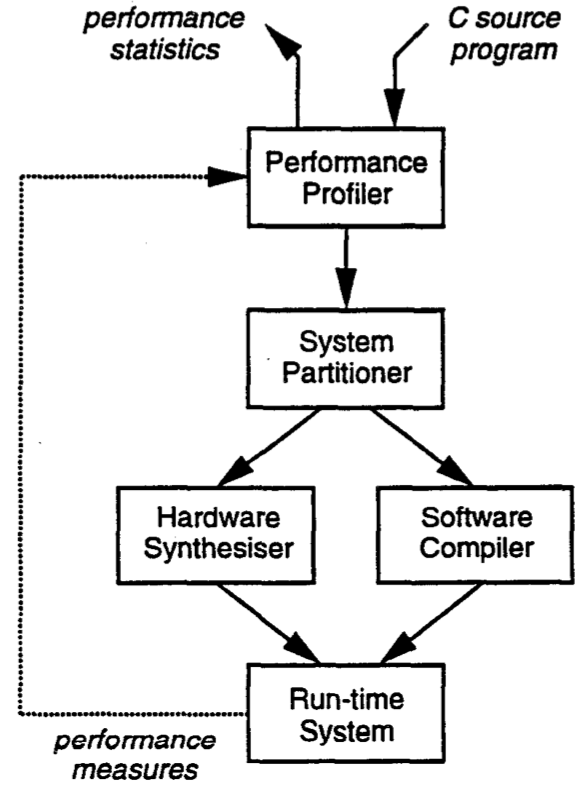
\includegraphics[width=0.8\textwidth]{img/rt-edwards_method.png}
\caption{Metodologia de \codesign. Fonte: \cite{Edwards1994}.}
\label{fig:tr-edwards_method}
\end{figure}
\end{column}
\end{columns}   

\pdfinfo{Tanto processos manuais, exatos ou heurísticos.}
\end{frame}

\begin{frame}{Pioneiro: \cite{Edwards1994}} \vspace{-1em}
\begin{itemize}
\setlength{\itemsep}{1.3em}
\item Utilizam do particionamento para aprimorar a performance do seu \software. 
\item Realiza-se a tentativa de tratar regiões críticas da aplicação 
\begin{itemize}
\item A solução em \software\ não pode chegar à restrições de performance requeridas;
\end{itemize}

\item Apresenta-se uma metodologia para desenvolvimento \codesign.
\begin{itemize}
\setlength{\itemsep}{1.0em}
\item Consiste na construção do código da aplicação em \textit{C} e sua análise;
\item Regiões críticas são identificadas e particionadas. 
\end{itemize}

\item Feito isso, realizar-se mensurações
\begin{itemize}
\item  Um novo particionamento é feito.
\end{itemize}

\item Utiliza-se de um FPGA.
\end{itemize}
\end{frame}

\begin{frame}{Trabalhos com Foco em Otimizações} \vspace{-1em}
\begin{itemize}
\setlength{\itemsep}{1.2em}
\item \cite{Stitt2003} pioneiro no método de otimização \textbf{dinâmico}.

\item Processos:
\begin{enumerate}
\setlength{\itemsep}{0.8em}
\item Detecta a região de mais executada e;
\item Reimplementa-a em \hardware\ de FPGA.
\end{enumerate}

\item Afirmam isso vantagens comparado com abordagens tradicionais manuais.

\item Como Stitt, outros propuseram algoritmos \textbf{exatos} baseados em estratégias:
\begin{itemize}
\setlength{\itemsep}{0.8em}
\item \textit{Branch-and-Bound} \cite{Jigang2004, Mann2007, Strachacki2008};
\item Programação dinâmica \cite{Madsen1997, Wu2006} e;
\item Programação Linear inteira \cite{Niemann1997}.
\end{itemize}
\end{itemize}
\end{frame}

\begin{frame}{Trabalhos com Foco em Otimizações} \vspace{-1em}
\begin{itemize}
\setlength{\itemsep}{1.8em}
\item \cite{Nematbakhsh_theeffect} exame da relação entre o \textit{footprint} do FPGA e o \speedup\ do \software.
\begin{itemize}
\item FPGA utilizado na implementação de \textit{loops} e sub-rotinas críticas.
\end{itemize}

\item Abordagem direta utilizando ferramentas comerciais como \textit{Synopys' Nimble Compiler} e \textit{Proceler} para a facilitação do processo.

\item \cite{Yan2017} parte da otimização \textit{position disturbed particle swarm} com otimização invasiva de \textit{weed} como o método de particionamento \hs.
\end{itemize}
\end{frame}

\begin{frame}{\cite{Wang2016}} \vspace{-1em}
\begin{itemize}
\setlength{\itemsep}{1.7em}
\item ``Particionamento depende da exploração de caracterização, estimação e \design\ espacial das métricas de custo e performance sistêmica.''
\begin{itemize}
\item Citam o \codesign\ é tão complexo que a simplificação do particionamento só para duas partes não é suficiente para a representação do problema como um todo. 
\end{itemize}

\item Incluem parâmetros chave de \design\ e uso de recursos que deveriam ser incorporados à modelagem do sistema
\begin{itemize}
\item Considera a modelagem de incerteza para particionamento de sistemas com um conjunto melhorado de parâmetros para compartilhamento de recursos \hs.
\end{itemize}

\end{itemize}
\end{frame}

\begin{frame}{\cite{Wang2016}} \vspace{-1em}
\begin{itemize}
\item Esse terceiro item a ser considerado ao problema de particionamento podem ser definidos em três tipos, sendo esses:
\begin{enumerate}
\setlength{\itemsep}{1.5em}
\item \textbf{Conjunto de recursos necessários para particionar uma dada tarefa:} sendo esses RAM, ROM, DPS, blocos IP do inglês, \textit{intelectual propriety}, entre outros; 
\item \textbf{Parâmetros de configurações que provê diferentes \textit{trade-off} entre recursos e performances:} exemplo circuitos de multiplicações sintetizados ou não;
\item \textbf{Dificuldade da mensura de desempenho e impacto no uso de recursos em várias configurações de partição com precisão precisando ter em mente a partição com a natureza incerta\footnote{Teoria da incerteza: Matemática axiomática para modelagem de graus de crença.} dessas estimativas não precisas.}
\end{enumerate}
\end{itemize}
\end{frame}

%\frame{\centering \bf \Huge \color{beamerCinza} Sistemas Embarcados}   

\begin{frame}{Embarcados} \vspace{-1em}
\begin{itemize}
\setlength{\itemsep}{1.8em}
\item SE é amplamente pesquisado desde 90 \cite{Ernst1993, Gupta1995, Hardt1995, Gajski1994, Bolsens1997}.

\item \cite{Mei2000} Descreve um particionamento além de uma abordagem de escalonamento para DRESs\footnote{Do inglês \textit{dynamically reconfigurable embedded systems}.}
\begin{itemize}
\item Para o escalonamento, \cite{Mei2000} Algoritmo Genético.
\end{itemize}

\item Contribuições
\begin{itemize}
\setlength{\itemsep}{1.0em}
\item Análise de tempo de configuração e;
\item Análise do tempo de reconfiguração parcial do FPGA.
\end{itemize}

\end{itemize}
\pdfnote{Embedded}
\pdfnote{reconfiguração parcial -> escalonamento p. de alocação restrita.}
\end{frame}

\begin{frame}{\cite{Arato2003}} \vspace{-1em}
\begin{itemize}
\setlength{\itemsep}{1.8em}
\item Descreve versões diferentes do particionamento
\begin{itemize}
\setlength{\itemsep}{1.0em}
\item Sistemas de tempo-real e custo restringido respectivamente;
\item Fornece análise matemática formal do problema, provando que é $ \mathcal{NP} $-difícil.
\end{itemize} 

\item Utiliza 
\begin{itemize}
\setlength{\itemsep}{1.0em}
\item Programação linear inteira resolvendo de forma otimizada, e;
\item Outra utilizando GA com soluções próximas ao ótimo global.
\end{itemize}
\end{itemize}
\end{frame}

\begin{frame}{\cite{Mann2007}} \vspace{-1em}
\begin{itemize}
\setlength{\itemsep}{1.2em}
\item Descrevem uma primeira tentativa para um algoritmo exato, não heurístico, para o problema de particionamento. 

\item Implementa-se a estratégia \textit{branch-and-bound} como um \textit{framework}, permitindo o incremento de outros algoritmos. 

\item Realizaram investigações para incrementar a eficiência do algoritmo com as técnicas:
\begin{itemize}
\item \textit{Lower bounds based on LP-relaxation}, uma mecânica de inferência customizada, condições não-triviais necessárias baseadas num algoritmo \textit{minimum-cut}, e diferentes heurísticas com passos pré-otimizados. 
\end{itemize}

\item Demonstram que podem resolver problemas complexos em tempo razoável. 
\begin{itemize}
\item O resultado é em entorno de dez minutos mais rápido que algoritmos exatos anteriores baseados em programação linear inteira para os testes realizados.
\end{itemize}
\end{itemize}
\pdfnote{Prox slide: pesq mais recentes}
\end{frame}

\begin{frame}{\cite{Hassine2017}} \vspace{-1em}
\begin{itemize}
\setlength{\itemsep}{1.5em}
\item Aplicou otimizações sobre o tempo de execução e gasto energético.

\item O algoritmo proposto destina-se a alcançar um particionamento de grafos à procurar o melhor conjunto da relação energia e tempo de execução.

\item Comparou-se com \textit{Simulated Annealing}, Busca Tabu e Genético
\begin{itemize}
\item Mostra-se mais adequado para aplicações em \cores\ de sistemas embarcados que necessitam do equilíbrio no \textit{tradeoff} de sistemas embarcados.
\end{itemize}

\end{itemize}
\end{frame}

\begin{frame}{\cite{Trindade2016}} \vspace{-1em}
\begin{itemize}
\setlength{\itemsep}{1.8em}
\item Utiliza do GA para solucionar o problema.

\item Propõe novas abordagens usando técnicas de verificação baseadas nas teorias de módulo de satisfação (SMT, do inglês \textit{satisfiability modulo theories}). 

\item Apresentam um exemplo de particionamento, modelam e solucionam-o usando três diferentes técnicas
\begin{itemize}
\setlength{\itemsep}{1.0em}
\item A ideia principal é aplicar o método de verificação SMT ao particionamento, e;
\item Comparar os resultados com otimizações tradicionais como ILP e GA.
\end{itemize}

\end{itemize}
\end{frame}


\begin{frame}{\cite{Jozwiak2017}} \vspace{-1em}
\begin{itemize}
\setlength{\itemsep}{0.7em}
\item Seu \textit{survey} considera os aspectos de uma aplicação embutida
\begin{itemize}
\item Tecnologias de \design\ com foco sistemas móveis modernos e \wearables.
\end{itemize}

\item Cita-se dois paradigmas de desen. para SE sobre sistema de multi-processadores heterogêneos. O paradigma de sistemas 
\begin{itemize} \setlength{\itemsep}{0.5em}
\item \textbf{\textit{Life-inspired}:} 
\begin{itemize}
\item Especifica princípios, características e organização funcional e estrutural de SE com analogia à vida de um organismo inteligente;
\item Soluções de mecanismos e arquiteturas de sistemas para sua implementação. 
\end{itemize}

\item \textbf{\textit{Quality-driven}:} 
\begin{itemize}
\item Solução para o \design\ de disp. que necessitam de exigências de \textit{real-time}, baixo consumo de energia, entre outros; 
\item Dessa forma, especifica-se qual a nova qualidade do sistema a ser requeria e como esta meta é obtida. 
\item ``Define-se \textit{qualidade} de uma solução sistêmica proposta como o \textit{total de sua eficácia}\footnote{Grau em que uma solução atinge seus objetivos.} \textbf{e} \textit{eficiência\footnote{Grau em que uma solução usa recursos para realizar seus objetivos.} na resolução do problema real}''.
\end{itemize}
\end{itemize}

\end{itemize}
\pdfnote{ORIENTADO PELA QUALIDADE}
\pdfnote{juntas determinam o grau de EXCELÊNCIA}

\end{frame}


\begin{frame}{\cite{Jozwiak2017}} 

\begin{block}{Entretanto, descreveram ao final que \cite{Jozwiak2017}}
``Enquanto \designers\ aprenderam bastante na \textbf{construção} de plataformas de \hardware\ heterogêneos altamente paralelos, métodos e ferramentas automatizadas para a sua programação e o paralelismo do algoritmo, bem como o \codesign\ coerente da arquitetura \hs\ \textbf{ainda estão atrasados perante à tecnologia}''.
\end{block}
\end{frame}


\begin{frame}{\Wearable e FPGA}
\begin{itemize}
\setlength{\itemsep}{2em}
\item \cite{Plessl2003, Ahola2007, Abdelhedi2016, Narumi2016, Lee2015} que relacionam FPGAs com aplicação \wearable.

\item Entretanto, nenhum menciona análise metodológica do problema de particionamento \hs\ para \design\ de sistemas computacionais \wearables.
\end{itemize}
\end{frame}

\end{comment}



\section{Met1}


\begin{frame}{Grafo de Controle de Fluxo (GCF)}
\begin{itemize}
   \setlength{\itemsep}{1.6em}
   \item A decomposição de um DRS pode gerar dois componentes:
   \begin{itemize}
      \item Porção a ser realizada em \hardware\ e outra executada em \software;
   \end{itemize}
   
   \item Essa decisão de divisão é chamada de problema de particionamento.
   
   \item Para sistemas baseados em Plataformas FPGA, particionamento é um sub-problema de um problema mais geral localizado no \codesign, onde refere-se ao \design\ cooperativo.
\end{itemize}
\end{frame}

\begin{frame}

\begin{equation}
\gamma =
\frac{
   \text{\textit{hardware speed}}
}{
   \text{\textit{software speed}}
}
=
\frac{
   \frac{
      1
   } {
      \text{\textit{hardware time}}
   }
} {
   \frac{
      1
   }{
      \text{\textit{software time}}
   }
}
=
\frac{
   \text{\textit{software time}}
} {
   \text{\textit{hardware time}}
}
\end{equation}
\end{frame}


\begin{frame}{Ganho de Performance} \vspace{-1em}

\begin{eqnarray}
\Gamma (\mathbb{D}) & = &
\left [
1 + \sum _{i \in \mathbb{D}} \left (
\frac{
   p(i)
}{
   \gamma(i)
}-p(i)
\right)
\right ]^{-1} \\
\Gamma (\mathbb{D}) & = &
\left [
1 + \sum _{i \in \mathbb{D}} \left (
\frac{
   p(i)
}{
   \frac{s(i)}{h(i) + m(i)}
}-p(i)
\right)
\right ]^{-1} \label{eq:d_final}
\end{eqnarray}

\pdfnote{Cada membro contribui à performance do sistema.}
\pdfnote{D: os recurso em hardware}
\end{frame}

\end{document}
